\chapter{Experimental realization and validation}   \label{Chapter:experiment}
    
    
    Previously, Chapter\,\ref{Chapter:PMLSM design RSM} has compared and contrasted the suitability of \acf{PMLSM}, \acf{LFSM}, and \acf{LTFM} for \acf{NFJI} application. The evidence gathered indicates that \acs{PMLSM} out-perform \acs{LFSM} and \acs{LTFM} for the application described in Section\,\ref{Chapter:PMLSM design HM/design optimization/design citeria}. To move forward, there requires refinement and prototyping work in order demonstrate the superior performance of \acsp{PMLSM} in \acs{NFJI} applications when compared to \acfp{VCM}.  
    
    
% ===================================================================================================
% === NEW SECTION === NEW SECTION === NEW SECTION === NEW SECTION === NEW SECTION === NEW SECTION ===
% ===================================================================================================
\section{New requirements}                          \label{Chapter:experiment/requirements}
    
    To recall, the optimization problem translated from the requirement set in Section\,\ref{Chapter:PMLSM design HM/design optimization/design citeria} has the objective of finding a motor configuration that produces the highest jet velocity $v_{jet}$ given the power input $P$, the drug ampoule volume $V$, the motor mass $M$, and the total motor length $L_{motor}$. While being suitable for determining the best type of motor for \acs{NFJI} under some practical constraints, this optimization problem set does not aim to find the lightest motor that can produce \acsp{NFJI} at a fixed jet velocity $v_{jet}$. Therefore, we needed a problem description that is more appropriate for finding the lightest motor configuration capable of providing jet injections with a fixed volume $V$ and a fixed jet speed $v_{jet}$. This new requirement set demands:
    
    
    \begin{itemize}
        \item The device needs to deliver $V = 1\,\mathrm{mL}$ volume of fluid at a peak jet speed of $200\,\mathrm m/\mathrm s$ ($200\,\mathrm{\mu m}$ nozzle diameter),
        \item Theoretical peak power consumption $P$ at the peak jet speed to be less than $1.2\,\mathrm{kW}$ (the motor driver will consume more to overcome friction),
        \item The total length of the device should not exceed $20\,\mathrm{cm}$  (including the mechanical structure and ampoule),
        \item The motor mass $M$ must be minimized while the constraints above are applied.
    \end{itemize}
    
    
    The target jet speed of $200\,\mathrm{m/s}$ was chosen to be adequate to overcome viscous losses in drug injection orifices while leading to practical ($100\,\mathrm{m/s}$ to $150\,\mathrm{m/s}$) injection velocities\,\cite{mitragotri2006}, while the power consumption of $1.2\,\mathrm{kW}$ is within the capability of practical self-contained power sources and power electronic drives. The duration of a typical injection is $<0.5\,\mathrm{s}$, thus, heat dissipation during an injection is not taken into the design consideration list.
    

% ===================================================================================================
% === NEW SECTION === NEW SECTION === NEW SECTION === NEW SECTION === NEW SECTION === NEW SECTION ===
% ===================================================================================================
\section{Design concept}                              \label{Chapter:experiment/design concept}

    
    
    The most basic components of a \acs{PMLSM} consists of the magnet array and the coil winding in individual phases, as shown in Fig.\,\ref{fig:chap/experiment/design concept/magnet_coil_iron}. The mechanical design concept requires the Halbach magnet array to fit inside a thin tube of austenitic stainless steel like in Fig.\,\ref{fig:chap/experiment/design concept/magnet_stainlessSteelTube}. The magnet array is enclosed inside the stainless steel because the surface of the tube is used as a low-friction sliding contact for the moving armature assembly. The moving armature assembly includes the coil windings, a cylindrical bobbin made out of PEEK, phase winding terminals, an winding terminal end cap, the iron shell, linear plastic bearings, as well as a translator end cap to attach the drug ampoule piston rod with o-rings for water tight sealing.  Fig.\,\ref{fig:chap/experiment/design concept/bobbin_iron_coil_piston.pdf} and \ref{fig:chap/experiment/design concept/moving_mechanism.pdf} render the moving armature assembly and how it placed in the hand-piece device. 
    
    \begin{figure}[h]
        \centering
        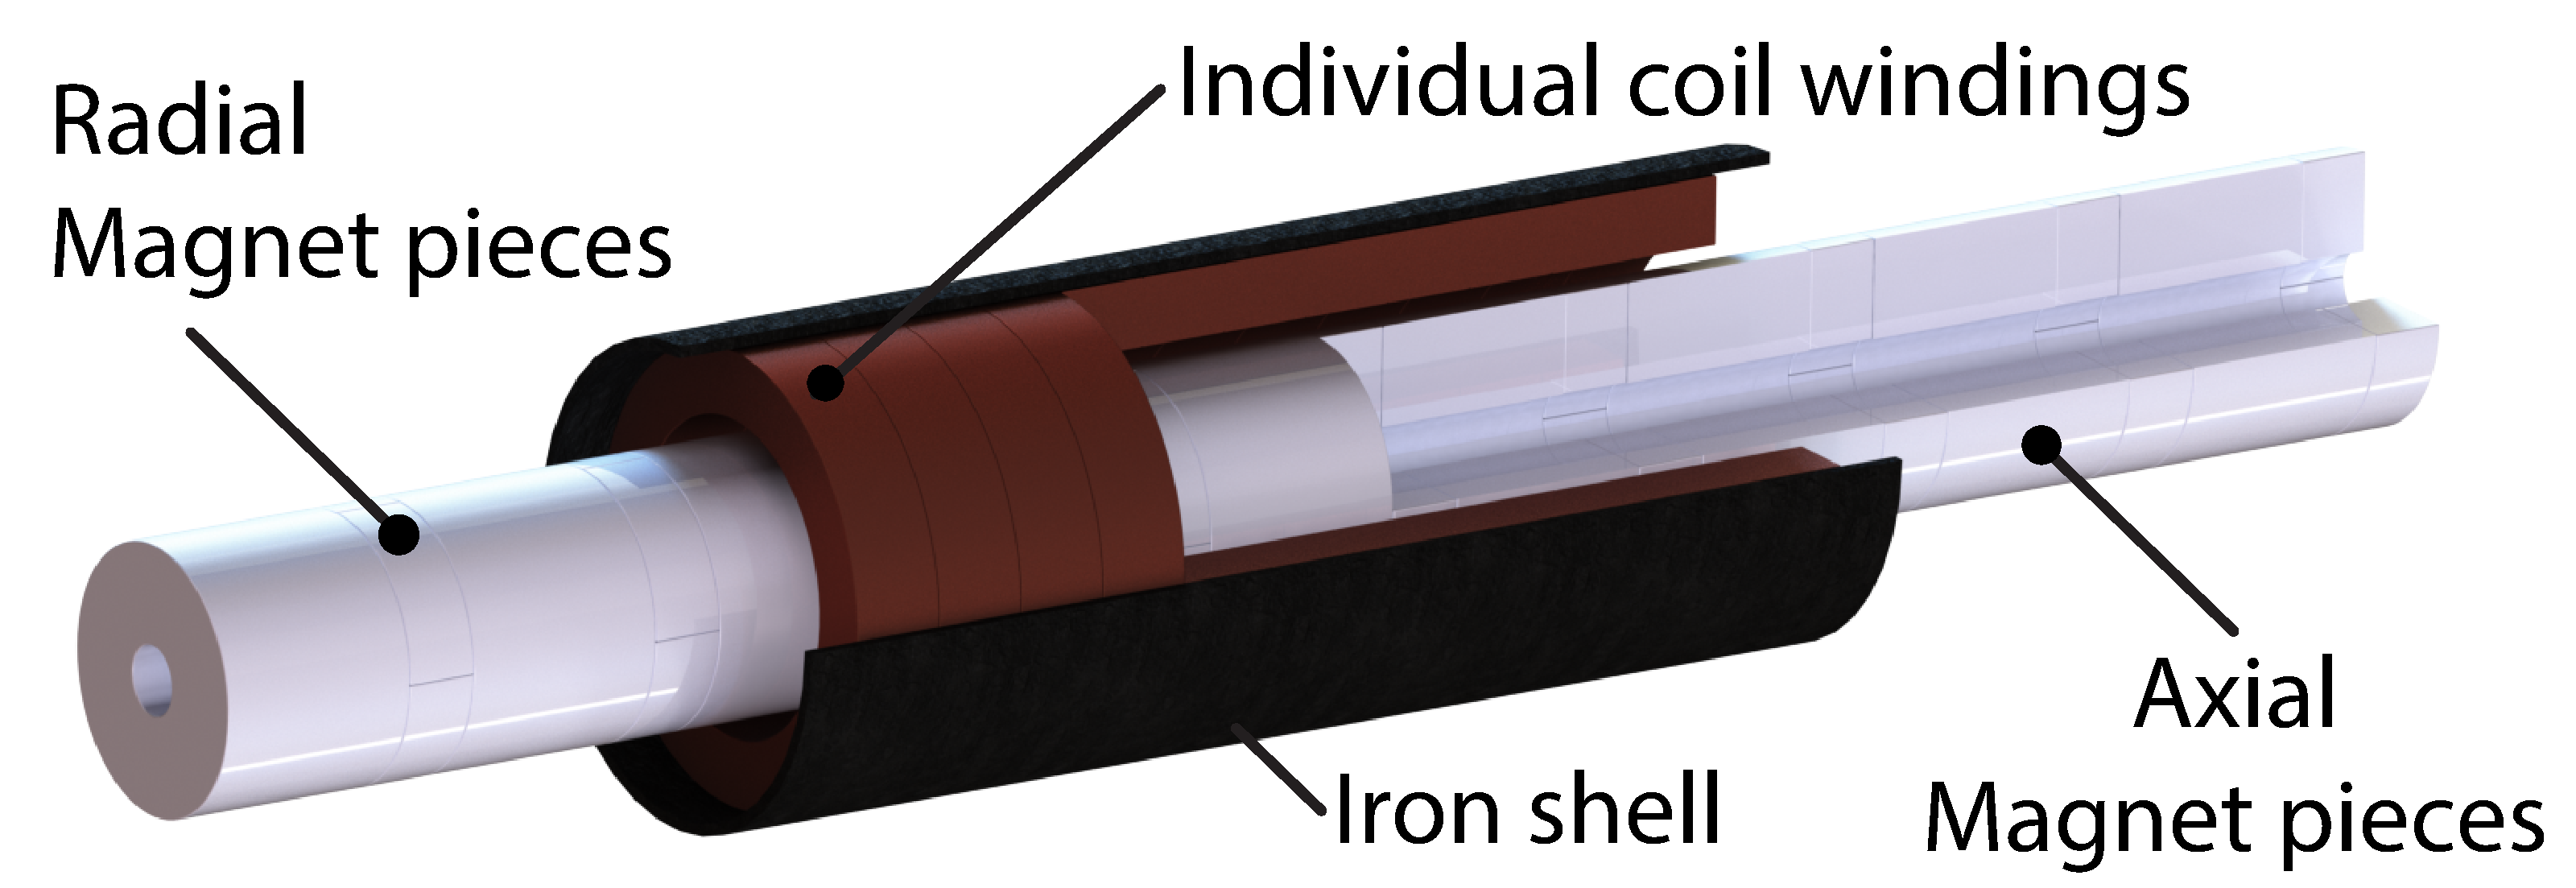
\includegraphics[width=3.8in]{chap5/images_concept/magnet_coil_iron.pdf}
        \caption{Render of the core elements for a PMLSM: the coil winding array, the magnet array, and the iron shell.}
        \label{fig:chap/experiment/design concept/magnet_coil_iron}
    \end{figure}
    
    
    \begin{figure}[h]
        \centering
        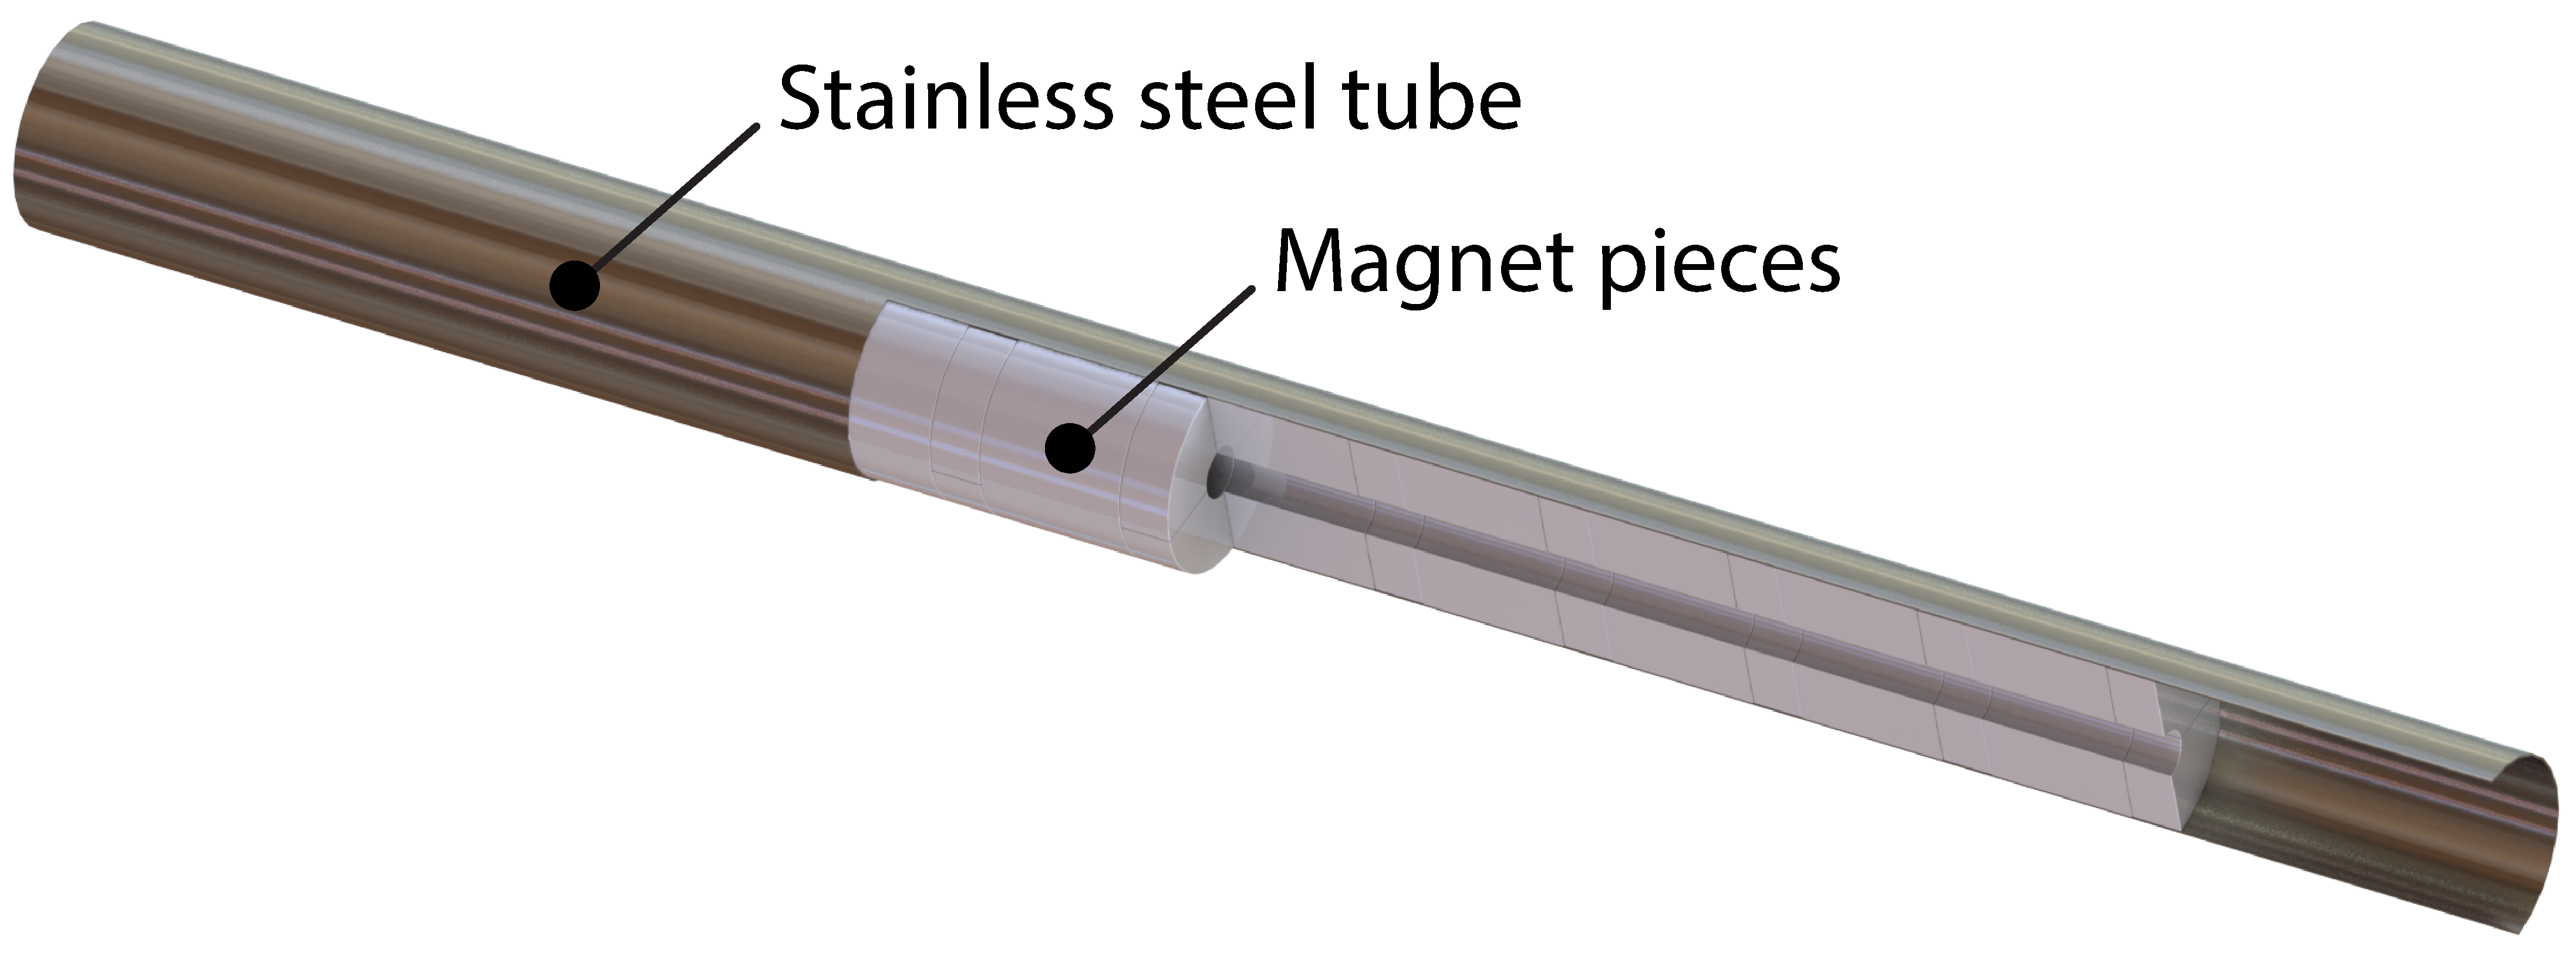
\includegraphics[width=4.2in]{chap5/images_concept/magnet_stainlessSteelTube.pdf}
        \caption{The magnet array is fitted inside a thin stainless steel tube with polished surface for minimum friction.}
        \label{fig:chap/experiment/design concept/magnet_stainlessSteelTube}
    \end{figure}
    
    
    \begin{figure}[h]
        \centering
        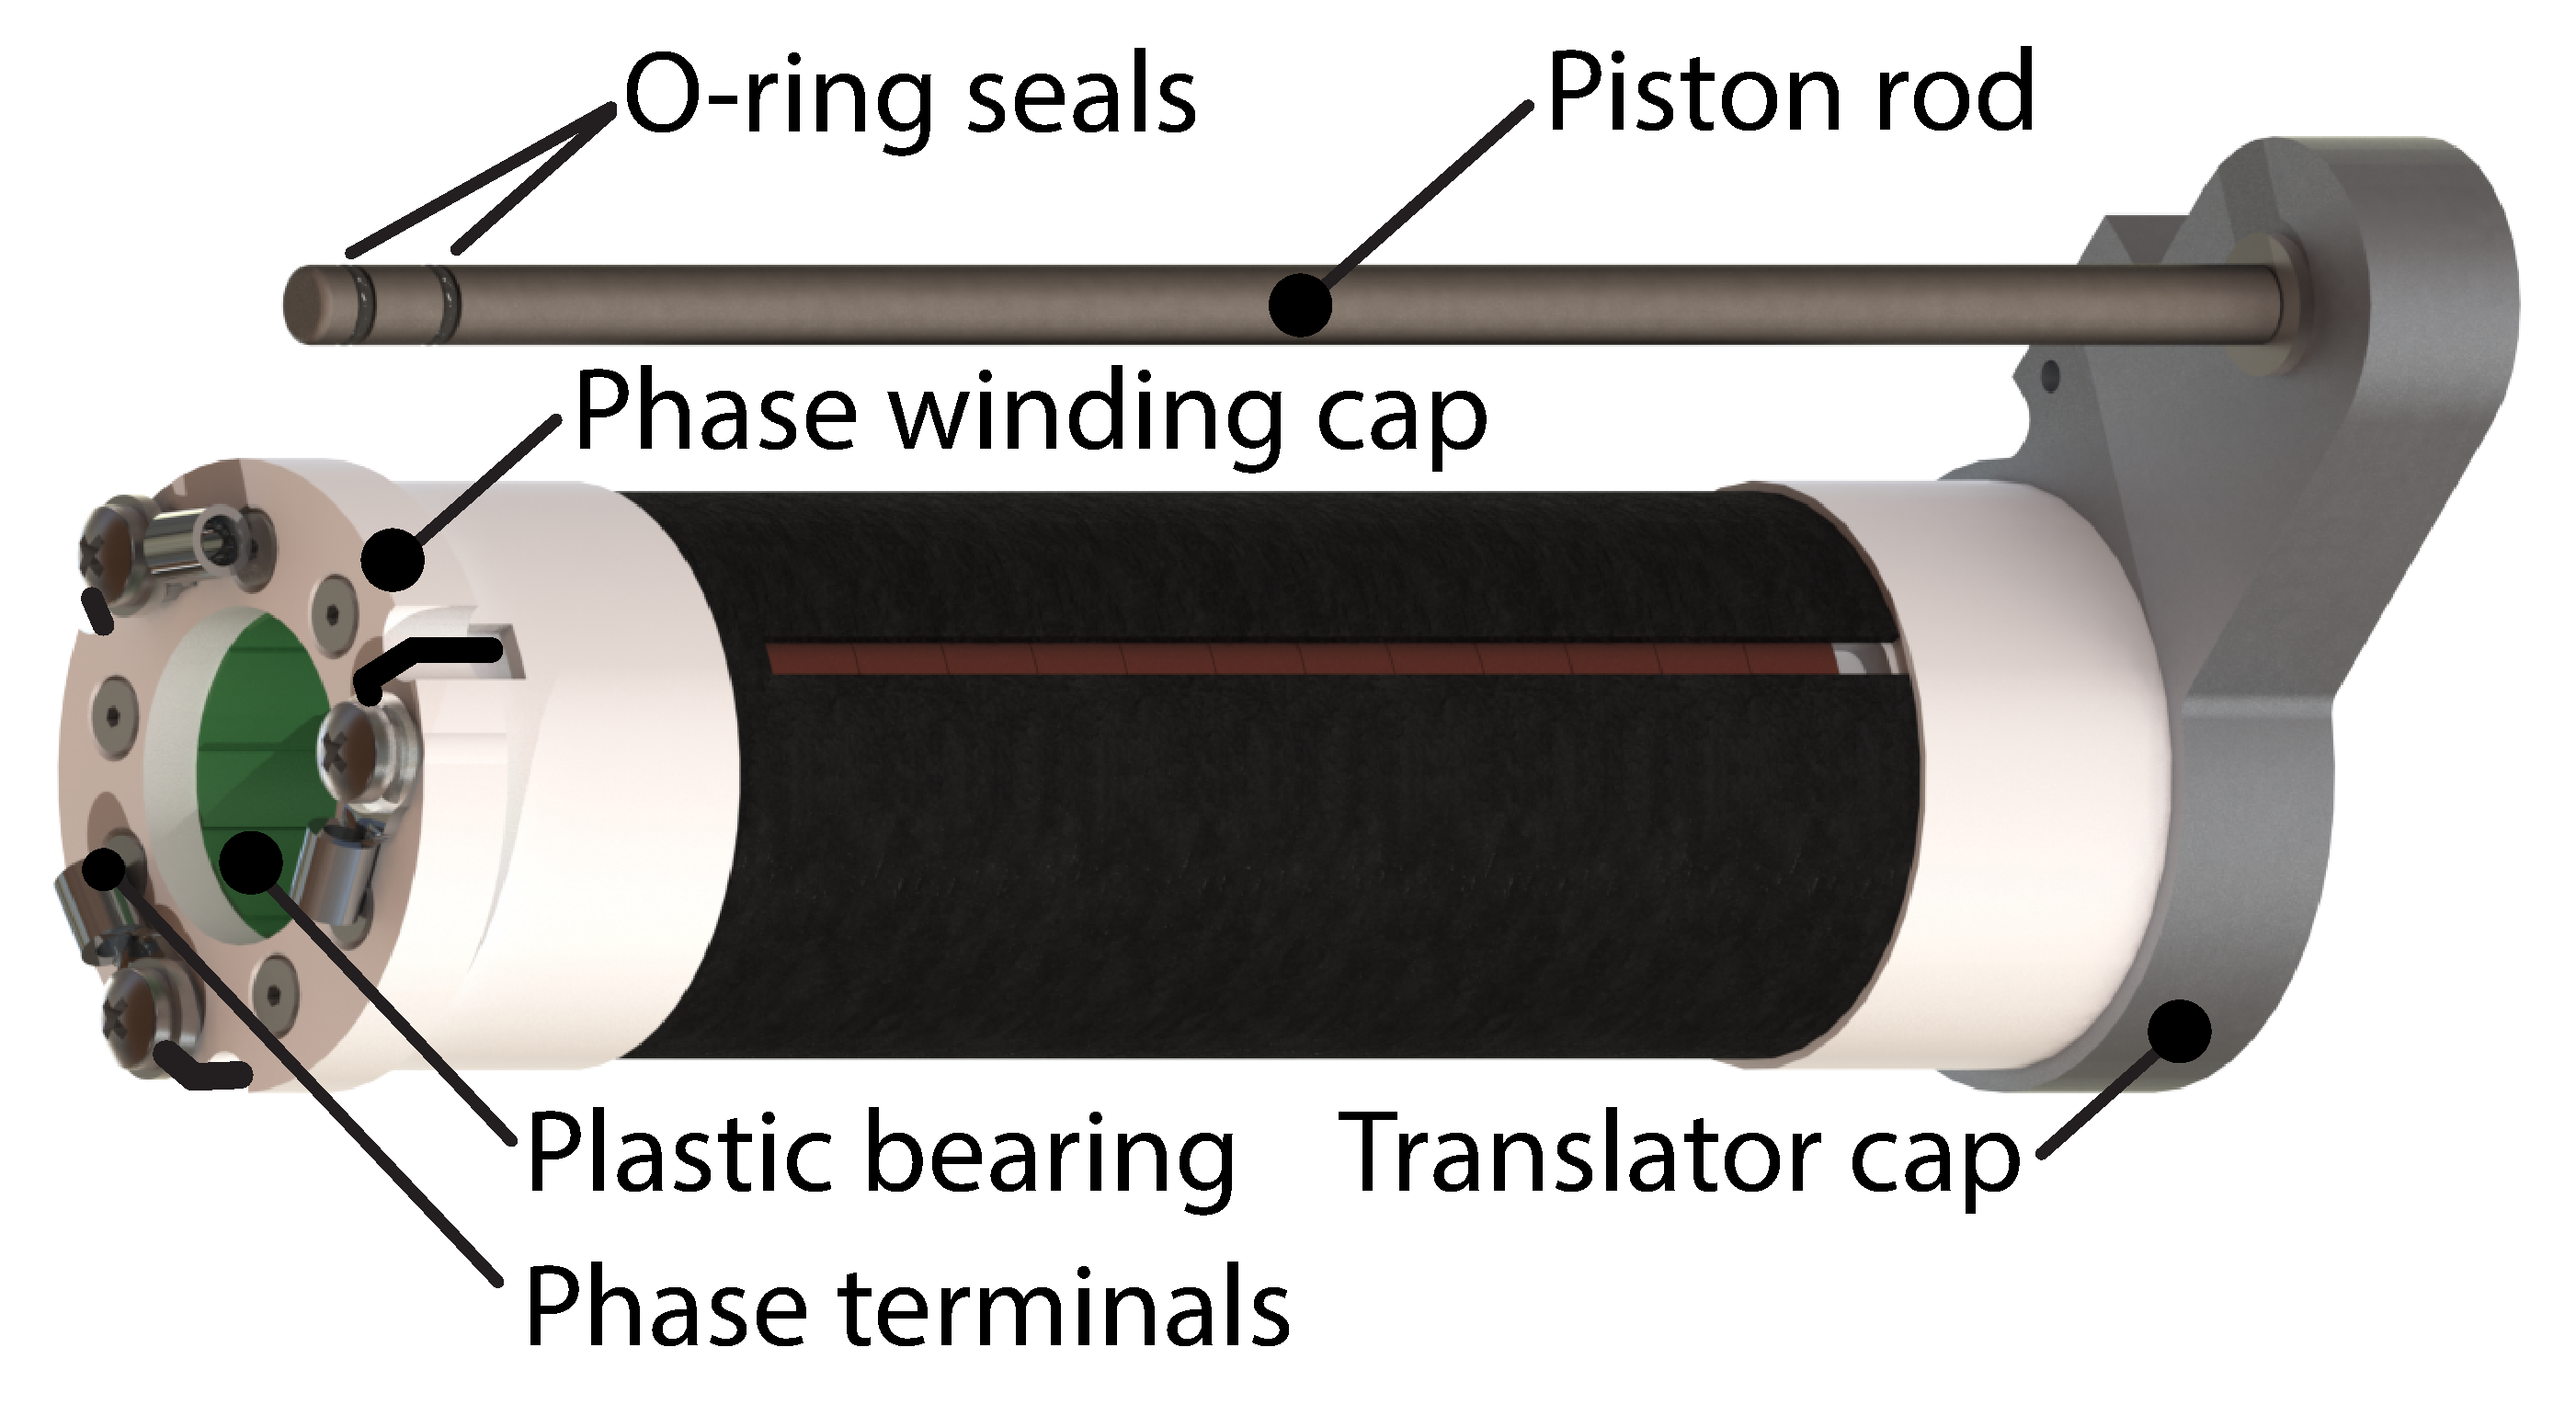
\includegraphics[width=3.3in]{chap5/images_concept/bobbin_iron_coil_piston.pdf}
        \caption{The moving armature assembly: coil windings, PEEK bobbin, phase terminals, plastic bearings, terminal end cap, translator end cap, and the drug piston rod with o-rings for water tight sealing.}
        \label{fig:chap/experiment/design concept/bobbin_iron_coil_piston.pdf}
    \end{figure}
    
    
    \begin{figure}[h]
        \centering
        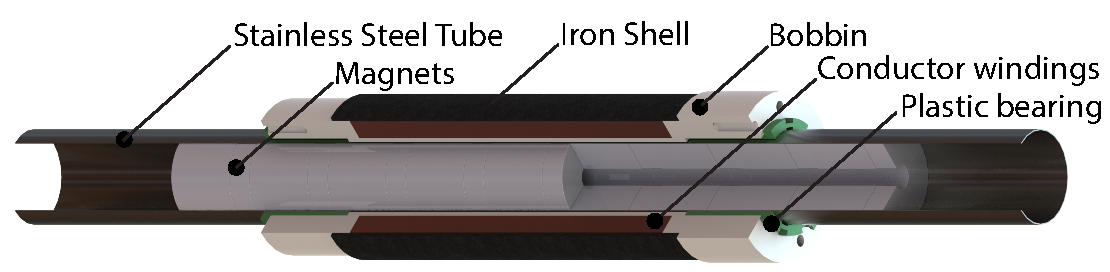
\includegraphics[width=5in]{chap5/images_concept/moving_mechanism.pdf}
        \caption{The stainless steel tube, the bobbin and the linear plastic bearings facilitate the sliding mechanism.}
        \label{fig:chap/experiment/design concept/moving_mechanism.pdf}
    \end{figure}
    
    
    As illustrated by Fig.\,\ref{fig:chap/experiment/design concept/magnet_stainlessSteelTube_endCap}, on two ends of the magnet tube, there are two enclosing reinforcement end caps held together by a threaded rod, nylon spacers (not shown), and tightened nuts (not shown). Together with the middle support plate and the nine support rods all made out of aluminium, the drug ampoule and nozzle are held precisely parallel with the core \acs{PMLSM} parts in Fig.\,\ref{fig:chap/experiment/design concept/magnetAssembly_supportStructure}. This design concept allows the total length of the motor to be shorter than placing drug ampoule in line with the magnet and armature assemblies. Now the actual length of the magnet array can be longer, which allows for higher performance motor designs. The support parts and the magnet end caps allow the whole motor structure to be extremely resilient against the axial moment left as translator end cap pushes the piston rod. Lastly, the frame of the motor incorporates a linear slide potentiometer as a position sensor, and a slide guide to couple the position of the armature assembly to the position of the slide knob. A cut view of the whole hand-piece is presented in Fig.\,\ref{fig:chap/experiment/design concept/full_cut_view_of_motor}.
    
    
    \begin{figure}[h]
        \centering
        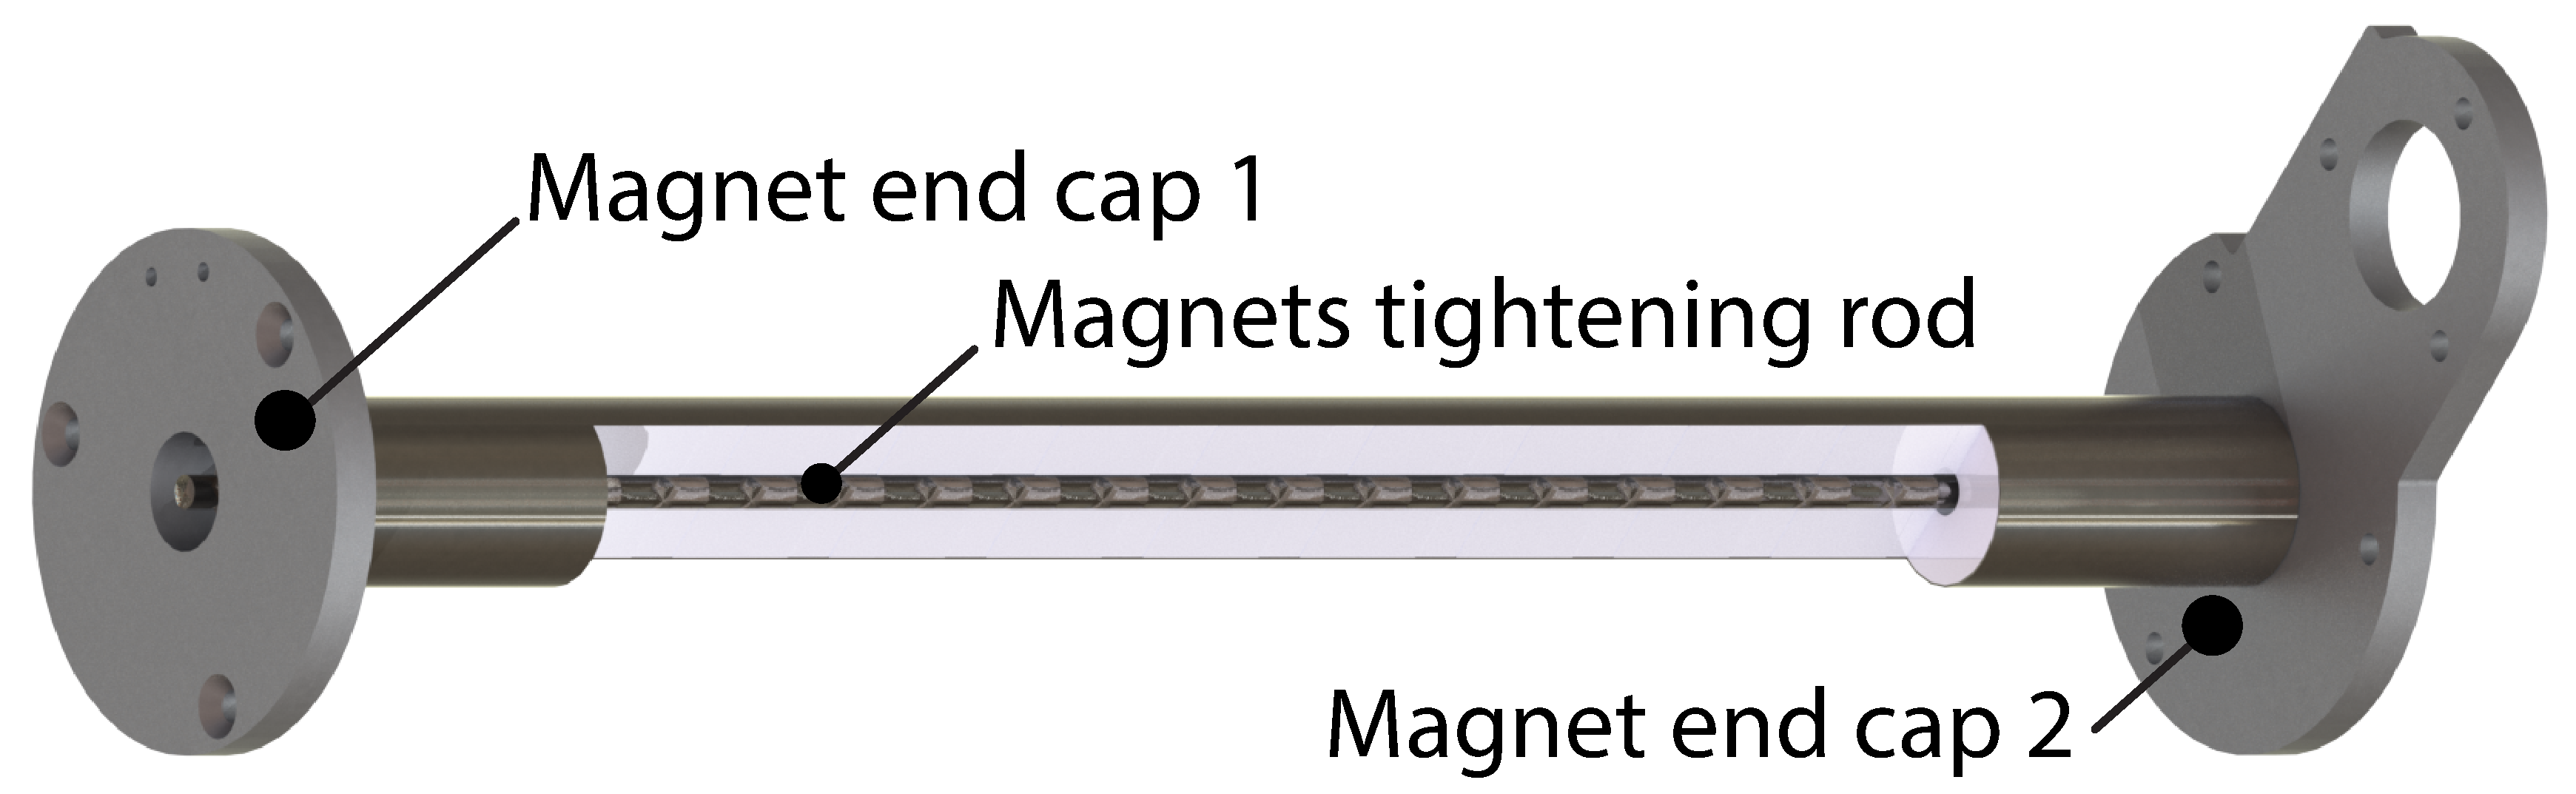
\includegraphics[width=4in]{chap5/images_concept/magnet_stainlessSteelTube_endCap.pdf}
        \caption{The magnet array is held in place by end caps, a threaded rod, nylon spacers (hidden), and tightening nuts on each end (hidden).}
        \label{fig:chap/experiment/design concept/magnet_stainlessSteelTube_endCap}
    \end{figure}
    
 
    \begin{figure}[h]
        \centering
        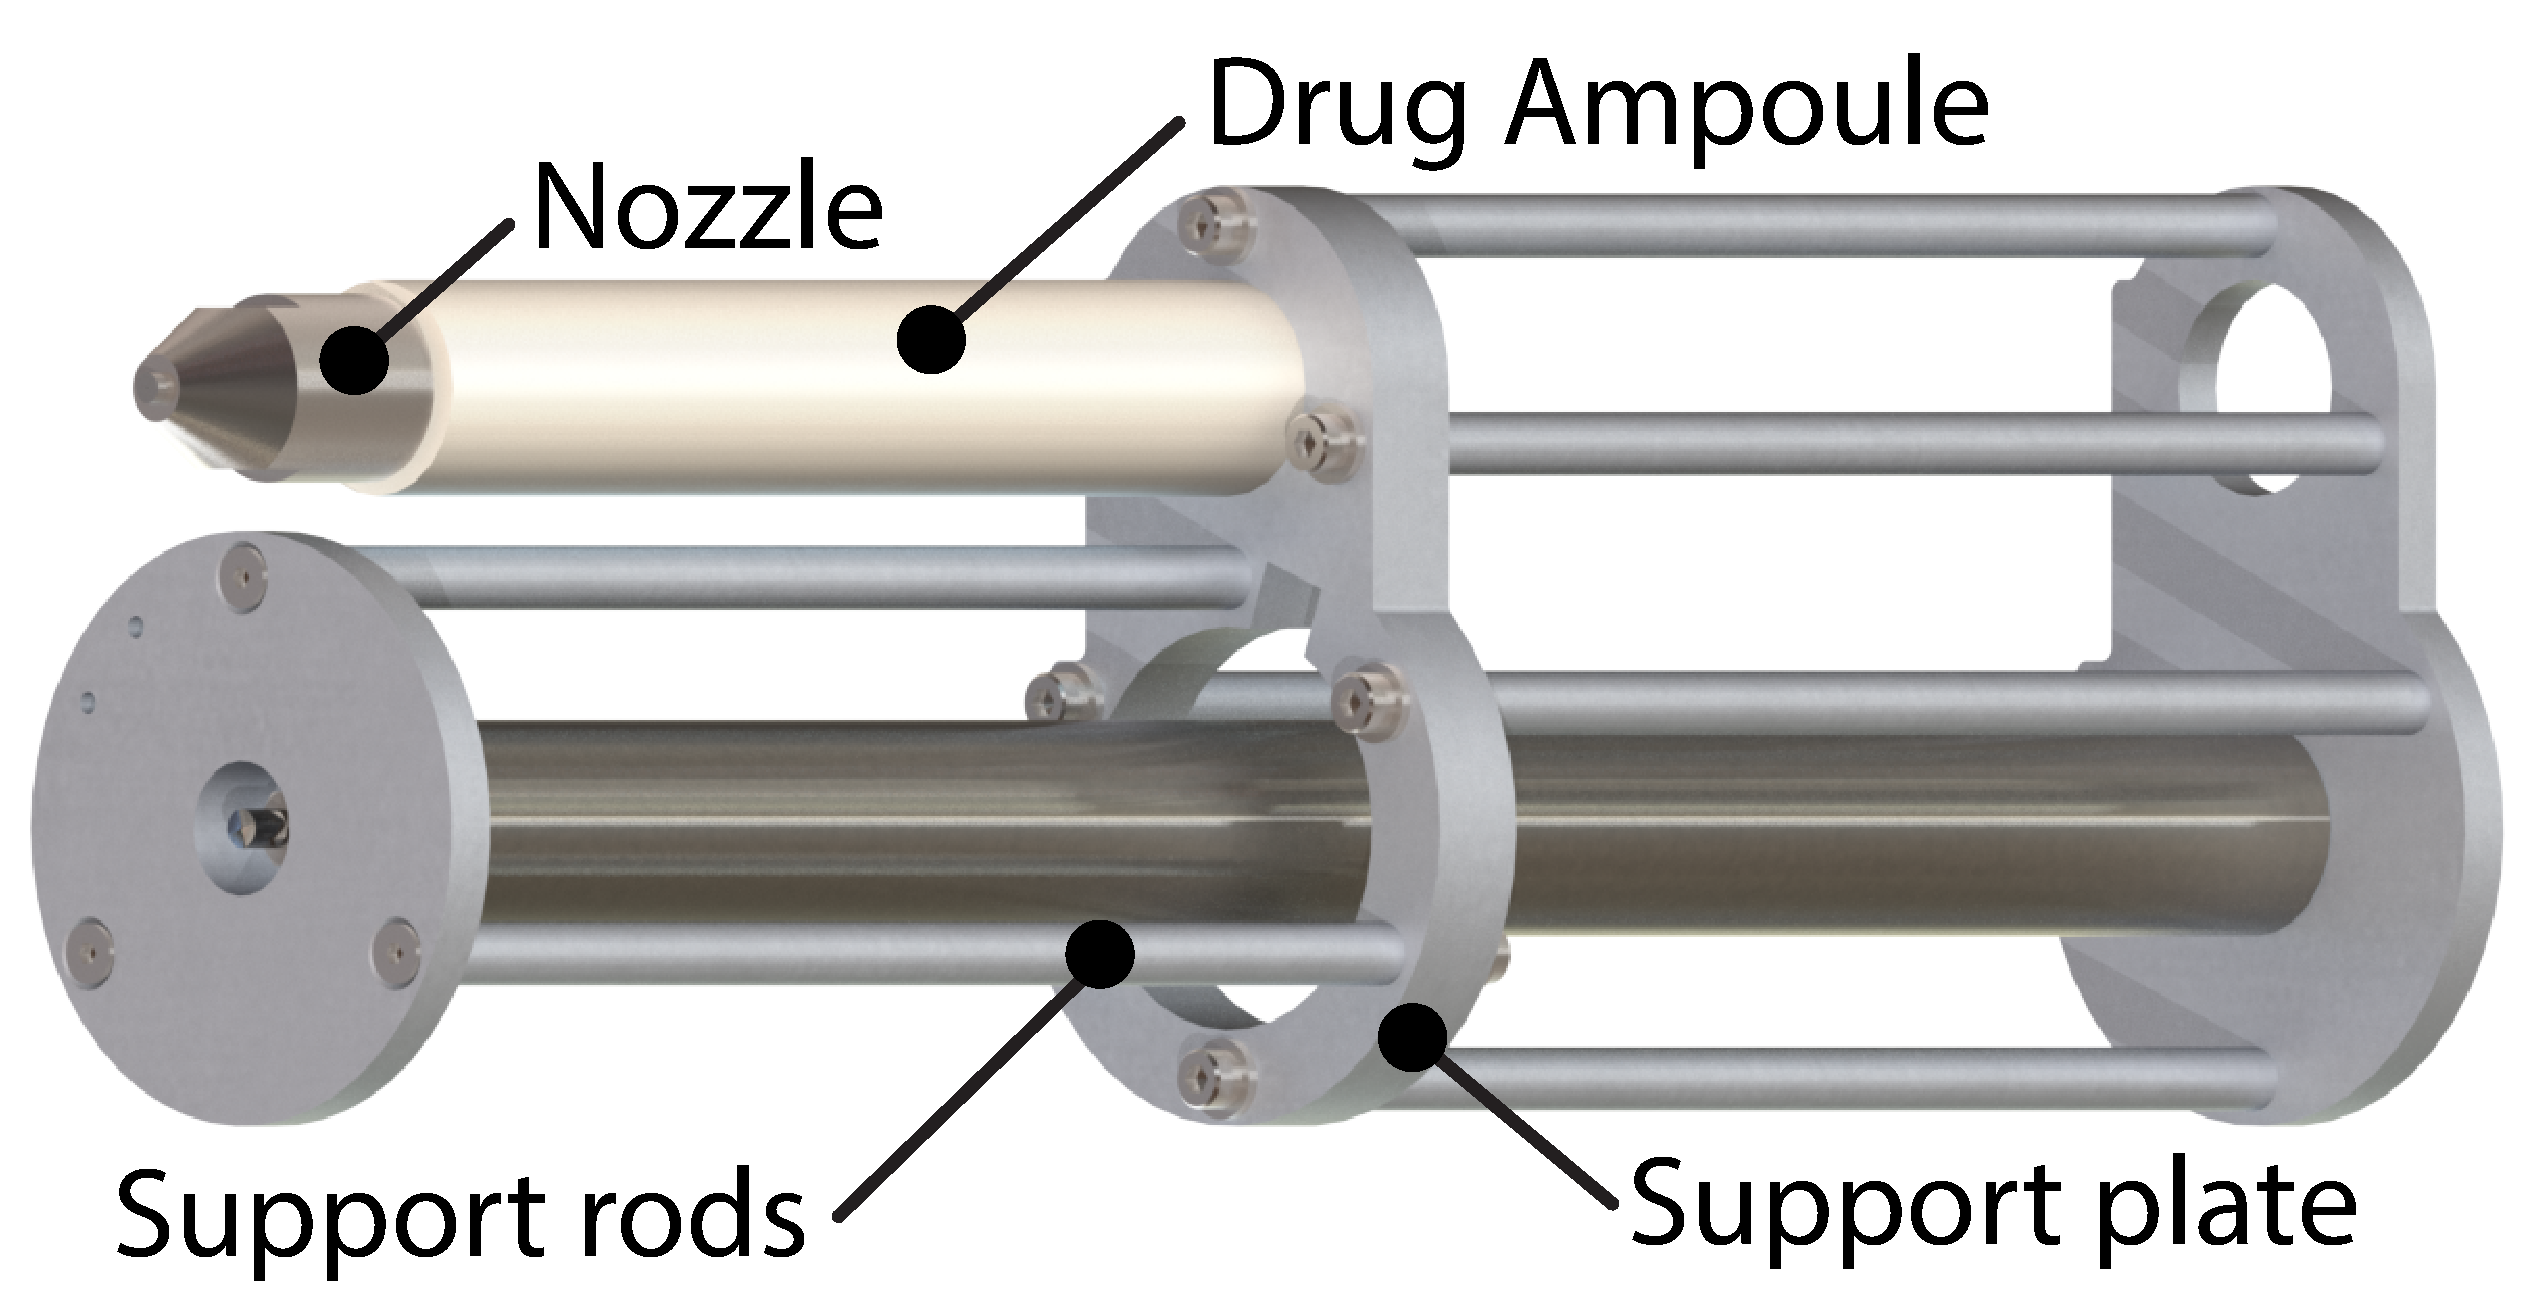
\includegraphics[width=3in]{chap5/images_concept/magnetAssembly_supportStructure.pdf}
        \caption{The magnet assembly, support structure and the drug ampoule assembly.}
        \label{fig:chap/experiment/design concept/magnetAssembly_supportStructure}
    \end{figure}
    
    
    \begin{figure}[h]
        \centering
        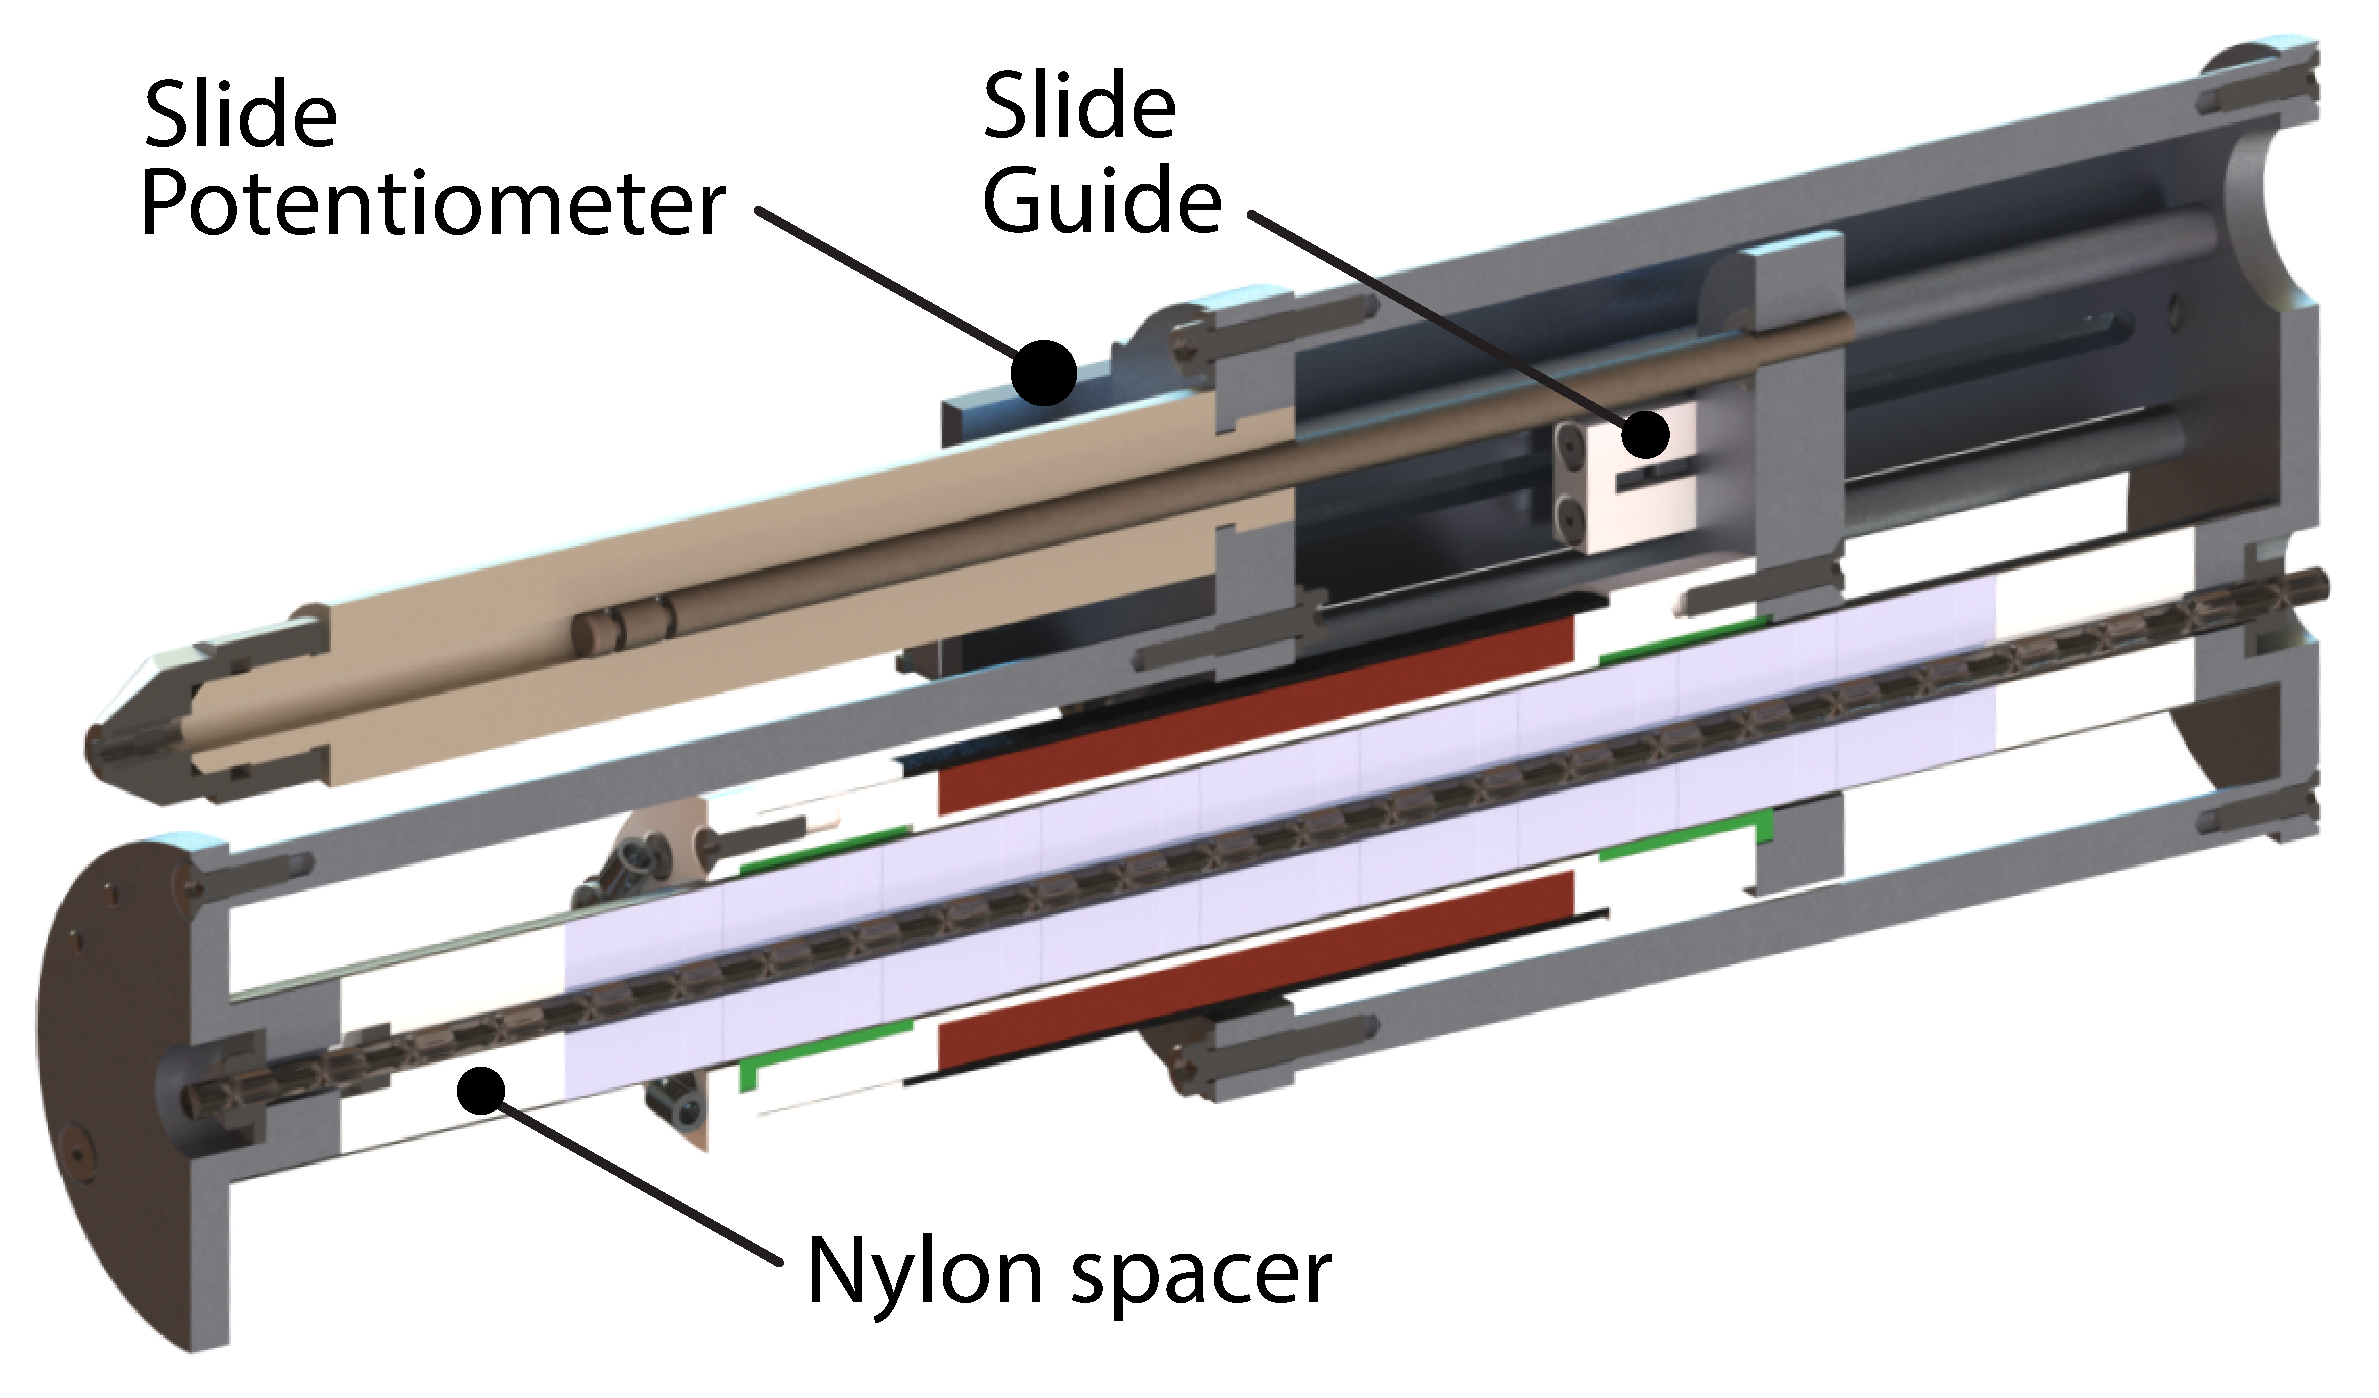
\includegraphics[width=4.5in]{chap5/images_concept/full_cut_view_of_motor.pdf}
        \caption{Cut view of the PMLSM hand-piece for high volume NFJI.}
        \label{fig:chap/experiment/design concept/full_cut_view_of_motor}
    \end{figure}


% ===================================================================================================
% === NEW SECTION === NEW SECTION === NEW SECTION === NEW SECTION === NEW SECTION === NEW SECTION ===
% ===================================================================================================
\section{Optimization}                              \label{Chapter:experiment/optimization}


    With the new set of design requirements established in Section\,\ref{Chapter:experiment/requirements}, an optimization scheme more suitable for finding the lightest motor with a list of fixed performance characteristics was realized. Based upon our previous development of power systems for jet injection \cite{Ruddy2017}, it was determined that the power electronics could support $1200\,\mathrm{W}$ of nominal motor power, with adequate margins, and with this new requirement, we focus on simultaneously minimizing the mass of the motor that would meet all the requirements. Since the number of half magnet-phase $N_M$ and half coil-phase $N_C$ were the only parameters subjected to integer constraints, each pair of $N_M$ and $N_C$ was treated as an independent non-linear optimization problem. In order to find a solution for this mixed-integer optimization problem, we used a method that can be divided into an outer optimization loop and an inner optimization routine.
    
    
    In a bird's eye view, the outer optimization loop executes a strategic repetition of the inner optimization routine. The inner optimization routine searches for the most power-efficient motor configuration at each given $N_{Mi}$, $N_{Ci}$, and $M_i$. The inner optimization problem is convex, and readily converges to a solution. The outer loop performs a grid search across a localized region in the ($N_M$, $N_C$) space, repeated around the optimum point until that optimum lies in the center of the search grid. This approach overcomes an observed lack of local convexity in terms of $N_M$ and $N_C$, by using a larger search grid than the scale of the non-convexity. This means that the program can gradually approach the best combination of $N_M$ and $N_C$ without getting stuck in numerous local minima. 
    
    
    Fig.\,\ref{fig:chap/experiment/optimization/illustraion of algo} summarizes and illustrates the optimization algorithm. The optimization problem is summarized as below:
    
    
    \begin{equation}
        \begin{array}{rll}
            \textbf{minimize}       & \small{objective\,\,function}     & f(\textbf{x})=M \\
            \textbf{subjected to}   & \small{equality\,\,constraint}    & h_1(\textbf{x})=d_s - d_{s0}= 0\\
                                    &\quad \small{where}                &\quad  d_{s0}\in\left[3,4,5\right]\,\mathrm{mm}\\
                                    &                                   & h_2(\textbf{x})=L_s - L_{s0} = 0\\
                                    &\quad \small{where}                &\quad  L_{s0}\in\left[140,80,50\right]\,\mathrm{mm}\\
                                    &                                   & h_3(\textbf{x})=V - 1\,\mathrm{mL} = 0\\
                                    &                                   & h_4(\textbf{x})=v_{jet} - 200\,\mathrm{m/s}=0\\
                                    & \small{inequality\,\,constraint}  & g_1(\textbf{x})=P - 1200\,\mathrm{W} \leqslant 0\\
                                            & \small{other\,\,constraint}       & N_C, N_M \in 	\mathbb{N} \\ \\
                \end{array}
                \label{eq:outer optimization for PMLSMs 2}
            \end{equation}    

    \begin{figure*}[h]
        \centering
        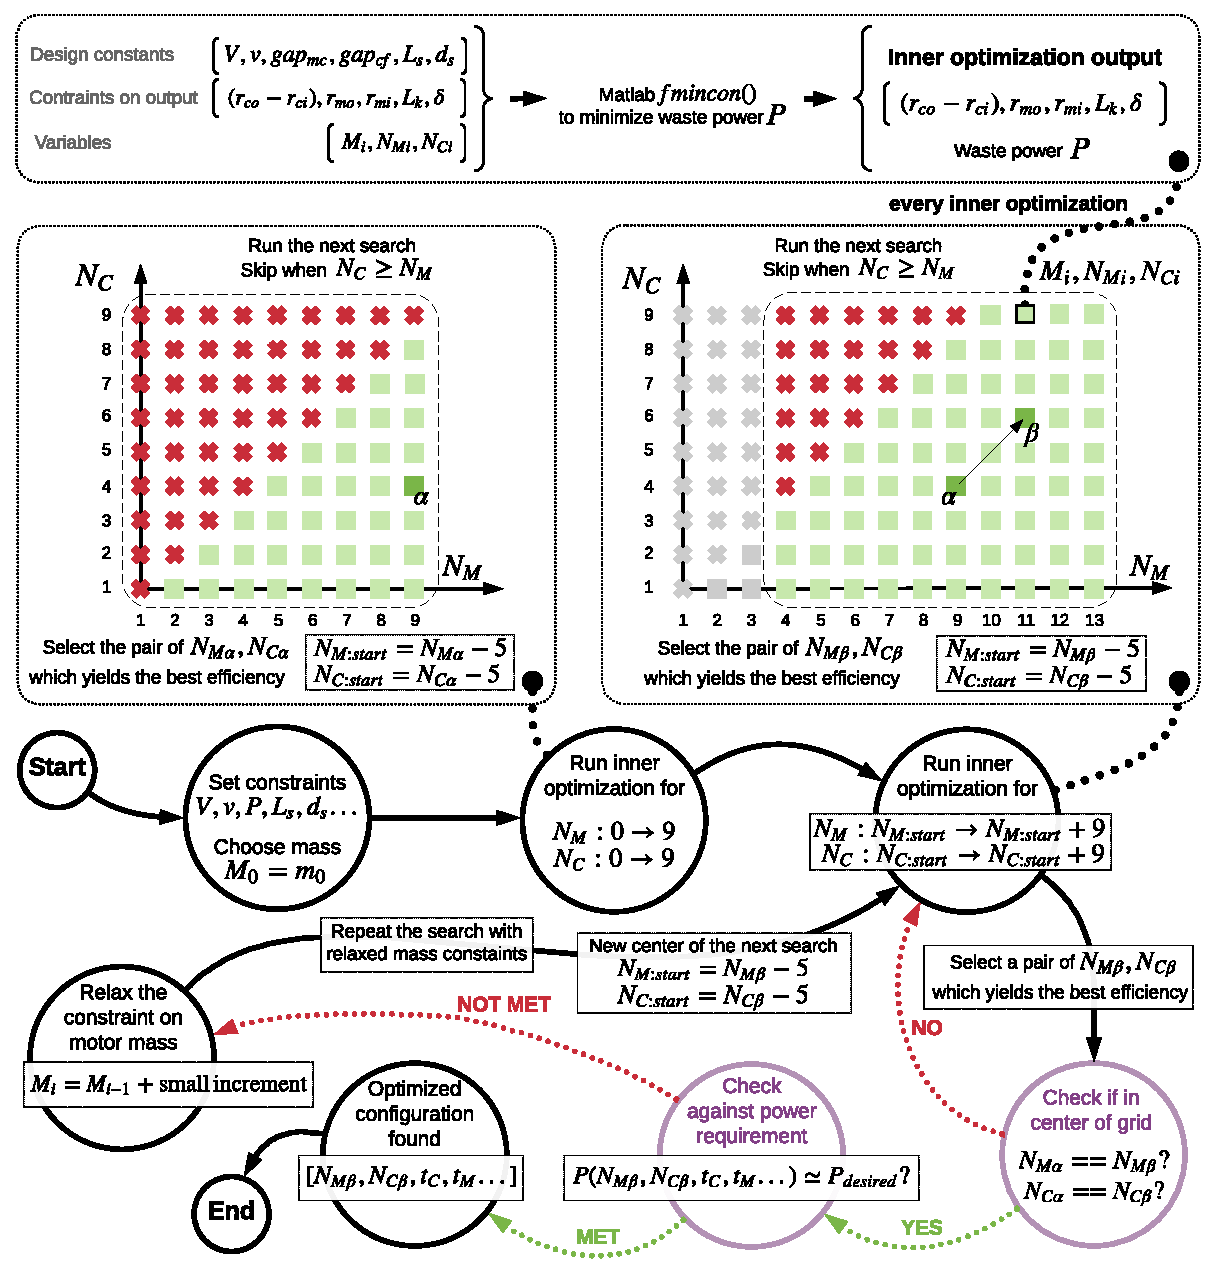
\includegraphics[width=5.8in]{chap5/images/optimization_illustration.pdf}
        \caption{Summary of the top-level motor optimization algorithm and inner optimization routine. The algorithm uses motor specifications $V$, $v$, $L_s$, and $P_{desired}$ to determine the motor parameters $L_k$, $r_mi$, $t_m$, $t_c$, $\delta$, $N_C$, $N_M$ and motor mass\,$M$ at which all specifications are satisfied.}
        \label{fig:chap/experiment/optimization/illustraion of algo}
    \end{figure*}
    
    
    In the very first round, the outer optimization routine first chooses an initial mass $M_0 = m_0$ and starts searching for the most power efficient motor that it can possibly achieve in the grid of $(N_M:0\rightarrow9)\times (N_C:0\rightarrow9)$. Each execution of outer optimization loop runs at most a hundred inner optimizations at a time in each grid search of $\left(N_{M:start}\rightarrow N_{M:start}+9\right)\times\left(N_{C:start}\rightarrow N_{C:start}+9\right)$, excluding overhung configurations (when $N_C \geq N_M$). After each grid search, the outer optimization loop identifies the most power efficient motor configuration so far to obtain the period numbers $N_{M\beta}$, $N_{C\beta}$. The search stops once this motor configuration with power consumption $P$ is found to be near enough to the desired power. If this motor configuration has not met the power requirement, the next grid search takes $N_{M\beta}$, $N_{C\beta}$ as its new center for the next grid search ($N_{M:start}=N_{M\beta}-5$, $N_{C:start}=N_{C\beta}-5$), and the $M_i$ set point in the outer optimization is increased by a small amount ($M_i=M_{i-1}+\mathrm{small\,increment}$). In this approach, the mass $M$ allowed in the motor search is increasing, while the power consumption $P$ of motor configurations found by inner optimization is decreasing to approach the desired power. 
    
    \begin{table}[h]
        \renewcommand{\arraystretch}{1.2}
        \caption{Summary of motor optimization constants and constraints}
        \label{table:chap/experiment/table of optimization value ranges}
        \centering
        \begin{tabular}{llr}
        \hline
        \bfseries Parameter & \bfseries Description & \bfseries Values\\
        \hline
        	$V$ 			& Maximum injection volume 				&	$1\,\mathrm{mL}$\\
            $v$				& Nominal jet speed						&	$200\,\mathrm{m/s}$\\
            $r_{co}-r_{ci}$	& Coil thickness 						&	$\geq4\,\mathrm{mm}$\\ 
            $r_{mo}$		& Fixed outer magnet array outer radius &	$7.8\,\mathrm{mm}$\\
            $r_{mi}$		& Magnet array radius 					&	$\geq2\,\mathrm{mm}$\\ 
            $gap_{mc}$		& Magnet and coil fixed radial gap 		&	$1.3\,\mathrm{mm}$\\ 
            $gap_{cf}$		& Coil and iron fixed radial gap 		&	$0.1\,\mathrm{mm}$\\ 
            $L_k$			& Period length	 						&	$\geq12\,\mathrm{mm}$\\
            $\delta$		& Ratio of radial magnet over a period	& 	$1> \delta >0$\\
        \hline
        	$N_M,N_C$		& Number of half magnet \& coil phases	&	$\in\mathbb{N}$\\ 
            $N_M-N_C$		& Underhung ($>0$) or Overhung ($<0$)	&	$>0$\\ 
            $M$				& Motor mass							&	$\leq350\,\mathrm{g}$\\ 
            $L_s/d_s$		& Stroke lengths and stroke diameter sets		&	$140\,\mathrm{mm}/\,3\,\mathrm{mm}$\\ 
            				& 										& 	$80\,\mathrm{mm}/\,4\,\mathrm{mm}$\\
                        	& 										& 	$50\,\mathrm{mm}/\,5\,\mathrm{mm}$\\
        \hline
        \end{tabular}
    \end{table}
    
    
    Due to the availability of parts, we constrained $r_{mo}=7.8\,\mathrm{mm}$ to allow the use of thin stainless steel tubing of $16\,\mathrm{mm}$ outside diameter. Furthermore, we chose to use standard precision austenitic stainless steel rods to reduce the machining work for the piston. Working back from the required volume $V$, the minimum stroke length $L_s$ is $140\,\mathrm{mm}$, $80\,\mathrm{mm}$, and $50\,\mathrm{mm}$ for piston diameter or ampoule inner diameter of $3\,\mathrm{mm}$, $4\,\mathrm{mm}$, and $5\,\mathrm{mm}$, respectively.
    
    
    We set the clearance gap between the magnet and coil $gap_{mc}\equiv r_{ci}-r_{mo} = 1.3\,\mathrm{mm}$, higher than the previously established value of $1.2\,\mathrm{mm}$,  to facilitate extra rigidity for the bobbin shell, and the gap between coil and back-iron $gap_{cf}\equiv r_{fi}-r_{co} = 0.1\,\mathrm{mm}$ to increase ease of assembly. Table~\ref{table:chap/experiment/table of optimization value ranges} summarizes the optimization constraints for the desired motor configuration. To reduce coupling between the radial dimensions, the thicknesses of the coil $t_c = r_{co} - r_{ci}$ and of the magnets $t_m = r_{mo} - r_{mi}$ were used in the optimization, instead of $r_{co}$ and $r_{mo}$. The five parameters for optimization were $L_k$, $r_{mi}$, $t_m$, $t_c$, and $\delta$. The parameters were also subjected to additional constraints: a minimum copper thickness of $\operatorname{Min}(t_c) = 4\,\mathrm{mm}$ to guarantee the structural integrity of the bobbin, outer magnet radii $r_{mo} = t_m + r_{mi} = 7.8\,\mathrm{mm}$ as noted above, a minimum inner magnet radius $\operatorname{Min}(r_{mi} ) = 2\,\mathrm{mm}$ to allow for structural support through the center of the magnet array, and minimum period length $\operatorname{Min}(L_k) = 12\,\mathrm{mm}$ to make coil winding more practical. A visualization for dimensions $t_c$, $t_m$, $gap_{cf}$, and $gap_{mc}$ are shown in Fig.\,\ref{fig:chap/experiment/design concept/additional_dimensions}.
    
    
    \begin{figure}[h]
        \centering
        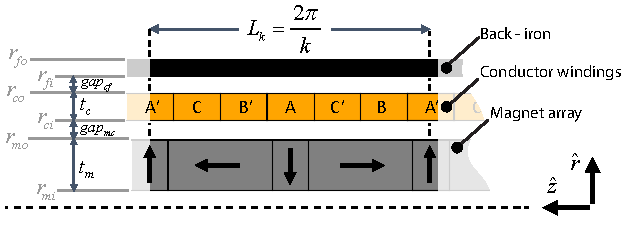
\includegraphics[width=5.6in]{chap5/images_concept/additional_dimensions.pdf}
        \caption{Coil thickness $t_c$, magnet thickness $t_m$, coil to iron gap $gap_{cf}$, and magnet to coil gap $gap_{mc}$ are shown.}
        \label{fig:chap/experiment/design concept/additional_dimensions}
    \end{figure}
    
    
    To gauge the performance of each motor design, the computation method outlined in Section \ref{Chapter:PMLSM design HM/electromagnetic model} is employed. The inner optimization routine uses constrained nonlinear multi-variable optimization based on the interior point algorithm (MATLAB Optimization Toolbox) to minimize power dissipation $P$, calculated via \eqref{eq:power dissipation for PMLSMs}, \eqref{eq:K_m}, and \eqref{eq:K_m dimless}. Many inner optimizations will be completed before the program can find the suitable motor. Across the inner optimization rounds, the following constraints are used: 
    
    
    \begin{itemize}
    \item Design constants such as injection volume $V$, jet speed $v$, $gap_{mc}$, $gap_{cf}$, stroke length $L_s$, and piston diameter $d_s$ are fixed;
    \item Constraints on the optimization output parameters ($L_k$, $r_{mi}$, $t_m$, $t_c$, and $\delta$) always apply;
    \item Variables such as $N_M$, $N_C$, and motor mass $M$ are up to the outer optimization loop to specify.
    \end{itemize}
    
    
    To see the effect of stroke length on the performance that can be obtained, Fig.~\ref{chap/experiment/optimization_result/different_stroke_length} plots $P_{max}$ against $M$ for three stroke lengths $L_s=50\,\mathrm{mm}/80\,\mathrm{mm}/140\,\mathrm{mm}$, using $V = 1\,\mathrm{mL}$, $v = 200\,\mathrm{m/s}$,  $P_{max} = 1.2\,\mathrm{kW}$ and other constraints. Although optimized motors with $140\,\mathrm{mm}$ stroke can offer superior performance given the same motor mass\,$M$, the overall motor length\,$L_{motor}$ required was found to be longer than $300\,\mathrm{mm}$. This result agrees strongly with the previous study in \cite{Ruddy2015a}: \acsp{PMLSM} can be more efficient if the motor length is allowed to be longer. However, with the ergonomics of the final handheld device in mind, only motors with $L_s = 80\,\mathrm{mm}$ appear to be feasible within both the motor mass and motor length limits stated in Table\,\ref{table:chap/experiment/table of optimization value ranges}. 
    
    
    \begin{figure}[h]
    \centering
    \subfloat[Minimum $M$ for given $P_{max}$ for different values of $L_s$]{
        \centering
        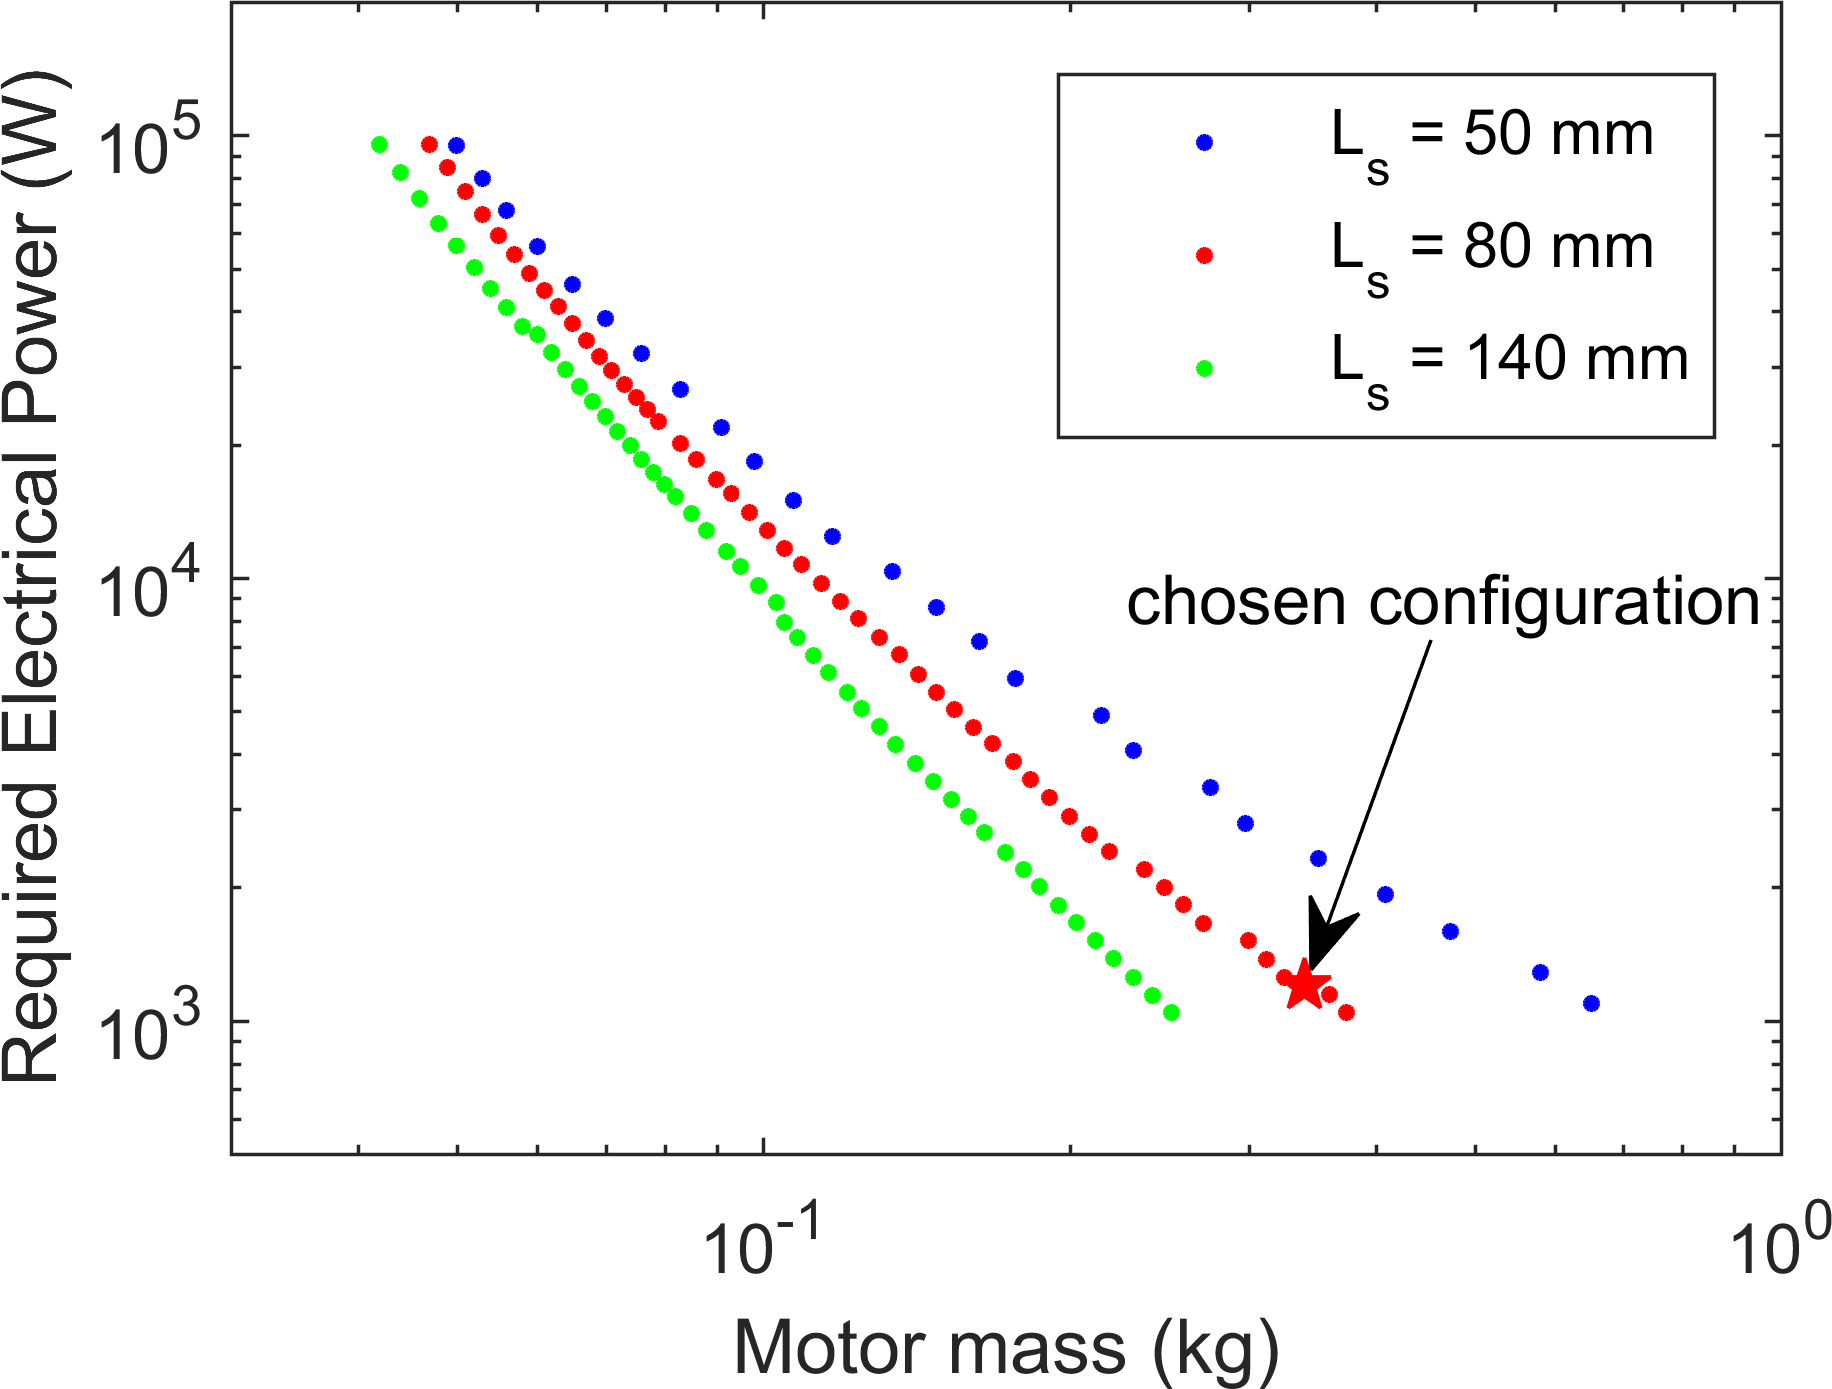
\includegraphics[width=3.4in]{chap5/images/different_stroke_length.png}
        \label{chap/experiment/optimization_result/different_stroke_length}
    }
    \\
    \subfloat[$N_M$ vs. $N_C$ search map]{
        \centering
        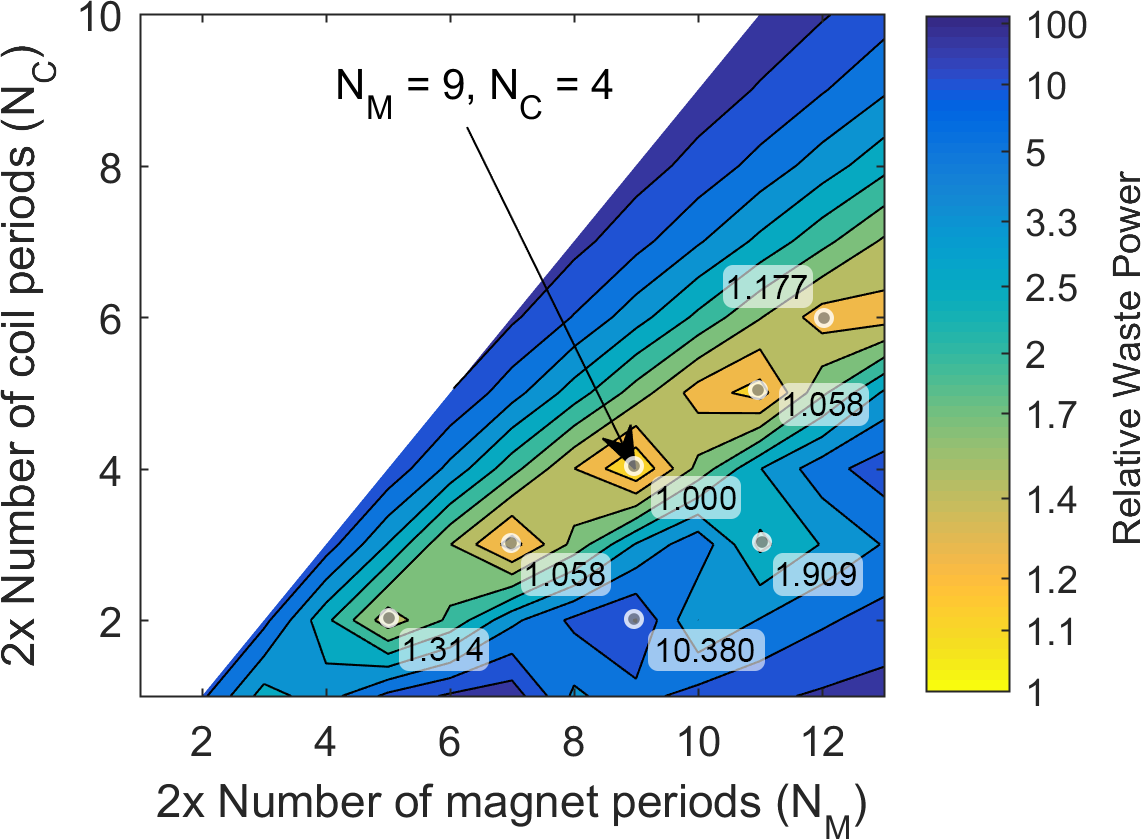
\includegraphics[width=3.4in]{chap5/images/phase_map.png}
        \label{chap/experiment/optimization_result/phase_map}
    }
    \caption{The $\left(N_{M:start}\rightarrow N_{M:end}\right)\times\left(N_{C:start}\rightarrow N_{C:end}\right)$  search map for a motor with $V = 1\,\mathrm{mL}$, $v = 200\,\mathrm{m/s}$,  $P_{max} = 1.2\,\mathrm{kW}$, and $L_s = 80\,\mathrm{mm}$ yields the least motor mass at $N_M = 9$ and $N_C = 4$ as shown in (a); and plot of $P_{max}$ against $M$ for different stroke length $L_s$ under the conditions $V = 1\,\mathrm{mL}$, $v = 200\,\mathrm{m/s}$,  $P_{max} = 1.2\,\mathrm{kW}$ (b). The chosen configuration for further cogging force optimization is labeled with a red star in (a), and annotated in both graphs. }
    \end{figure}


% ===================================================================================================
% === NEW SECTION === NEW SECTION === NEW SECTION === NEW SECTION === NEW SECTION === NEW SECTION ===
% ===================================================================================================
\section{Design selection}                          \label{Chapter:experiment/design selection}


    The global optimization for $V = 1\,\mathrm{mL}$, $v = 200\,\mathrm{m/s}$, $P_{max} = 1.2\,\mathrm{kW}$, and $L_s = 80\,\mathrm{mm}$ and stated constraints is an underhung motor with $N_C = 4$, $N_M = 9$, $L_k = 32\,\mathrm{mm}$, $r_{mi} = 2\,\mathrm{mm}$, $r_{mo} = 7.8\,\mathrm{mm}$, $r_{ci} = 9.1\,\mathrm{mm}$, $r_{co} = 13.1\,\mathrm{mm}$, $r_{fi} = 13.2\,\mathrm{mm}$, $r_{fo} = 13.93\,\mathrm{mm}$, $\delta = 0.258$ and $M = 322\,\mathrm{g}$. The plot in Fig.~\ref{chap/experiment/optimization_result/phase_map} illustrates that, at $N_C = 4$ at $N_M = 9$, the optimization algorithm found the most efficient motor configuration based on the input constraints. Furthermore, it appears to reach the optimization solution rather gradually and exhibit a noticeable degree of field convexity, which agrees with our assumption earlier.
    
    Considering a motor with $L_s = 80\,\mathrm{mm}$ acting upon a $1\,\mathrm{mL}$ ampoule with an orifice diameter of $200\,\mu \mathrm{m}$ to generate jet velocity of $200\,\mathrm{m/s}$, the motor is required to output $250\,\mathrm{N}$ at a stroke velocity of $0.5\,\mathrm{m/s}$. The analytical model estimates the dimensionless motor constant $\hat{K}_m$ to be $0.1107$, while the “single coil pole/single magnet pole” \acs{FEA} model, similar to that in\,\cite{Ruddy2011a}, is in strong agreement with the computed $\hat{K}_{m(FEA)}$ of $0.1149$. Upon fulfilling all requirements and \acs{FEA} validation, this motor configuration was chosen for further cogging force investigation before advancing to the final design.


% ===================================================================================================
% === NEW SECTION === NEW SECTION === NEW SECTION === NEW SECTION === NEW SECTION === NEW SECTION ===
% ===================================================================================================
\section{Cogging force reduction}                   \label{Chapter:experiment/cogging reduction}


    By design intention, the back-iron tube does not cover the whole length of the Halbach magnet array. Thus, the motor is prone to problems related to end effect cogging force such as control instability. To reduce the magnitude of the cogging force, an \acs{FEA} setup as illustrated in Fig.\,\ref{fig:/chap/experiment/cogging_force_optimization/Axisymmetric_FEA_model} was used to search for an alternative back-iron length that yields the least peak to peak cogging force. 
    
    \begin{figure}[h]
    \centering
    \subfloat[Cogging force optimization setup]{
        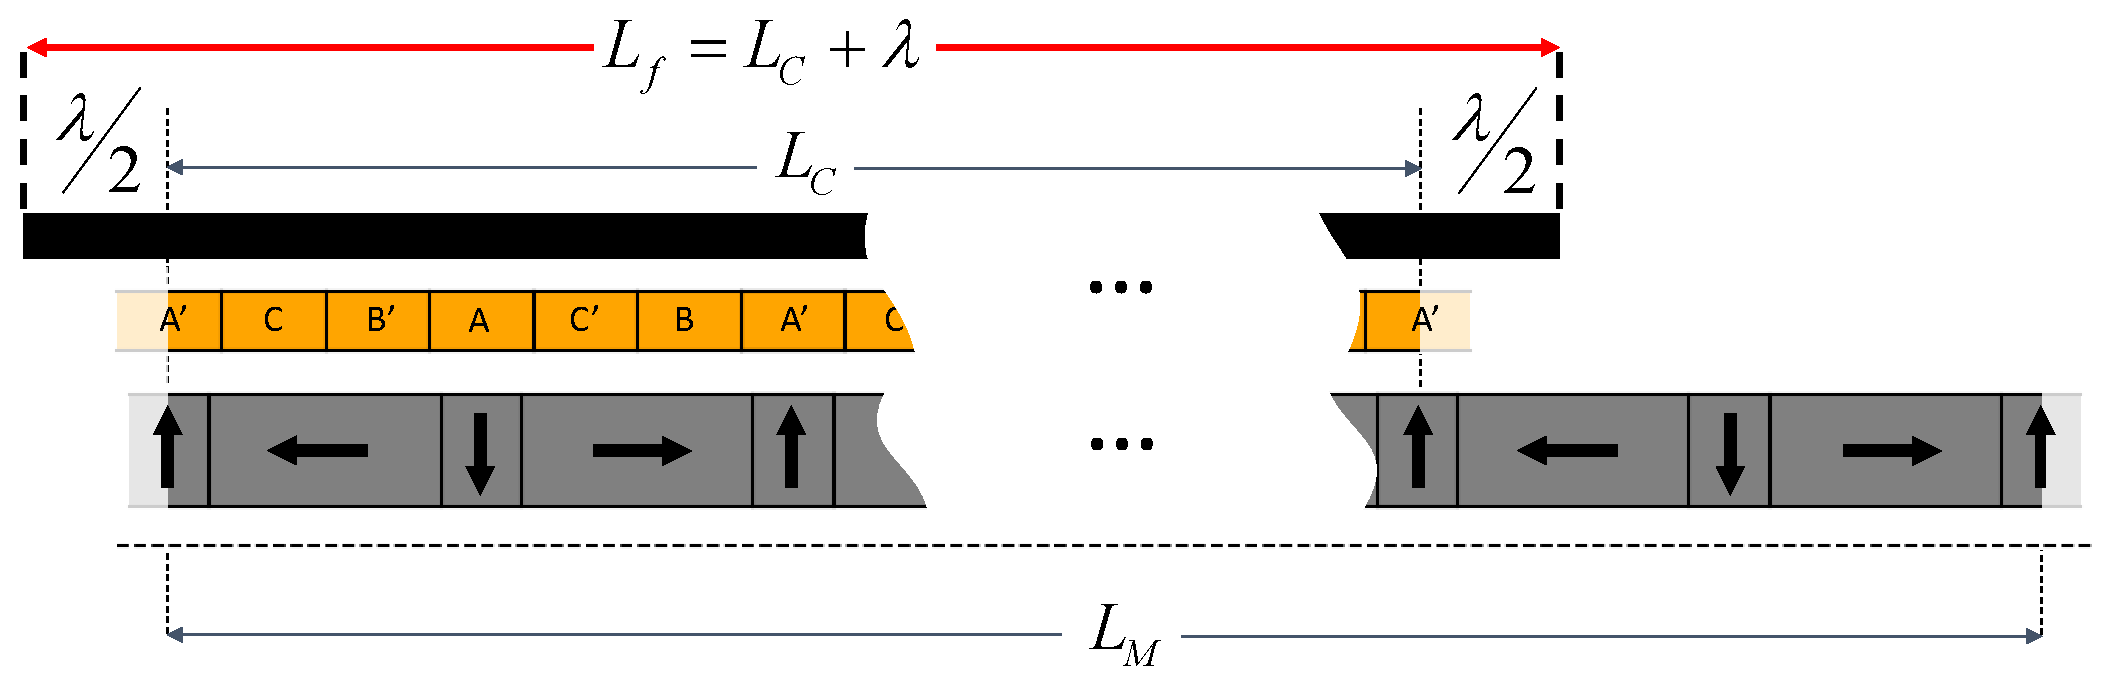
\includegraphics[width=4.5in]{chap5/images/cogging_optimization_setup.pdf}
        \label{fig:/chap/experiment/cogging_force_optimization/Cogging_optimization_setup}
    }
    \\
    \subfloat[Axisymmeic FEA model illustration]{
        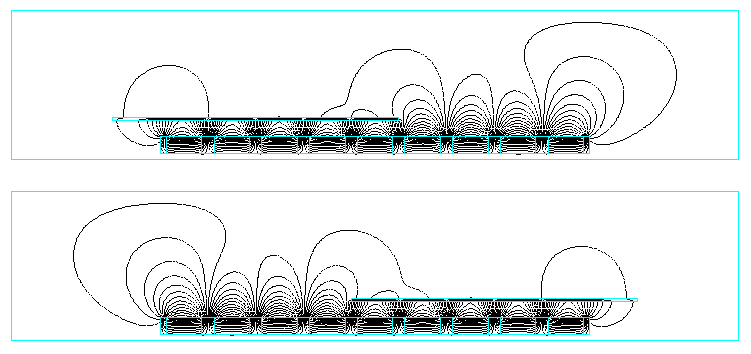
\includegraphics[width=4in]{chap5/images/cogging_FEA_setup.png}
        \label{fig:/chap/experiment/cogging_force_optimization/Axisymmetric_FEA_model}
    }
    \caption{Cogging force optimization with extended back-iron length $L_f = L_C + \lambda$, where $\lambda$ is extra back-iron length, $\Delta$ is motor axial position in (a); and axis-symmetric \acs{FEA} model to work out cogging force for each $L_f$ over the range of $\Delta  = 0 \rightarrow L_s$ with no applied current in (b).}
    \end{figure}
    
    
    The cogging force optimization process was started by creating a base ANSYS Mechanical APDL script that describes the motor configuration obtained from the previous optimization. The model included additional parameterization of sleeve length $\lambda$ and coil position $\Delta$ while excluding the conductor and input current conditions, as illustrated in Fig.~\ref{fig:/chap/experiment/cogging_force_optimization/Axisymmetric_FEA_model}. We created a Python automation script to collect axial forces acting on the back-iron $F_c$, then changed $\lambda$ and $\Delta$ accordingly to repeatedly call the APDL batch process for the same base script. The automation script split the job into 5-6 concurrent threads which called independent APDL batch processes to fully exploit the available computing power.
    
    
    \begin{figure}[h]
        \centering
        \subfloat[Searching for $L_f$ which yields the least cogging]{
            \includegraphics[width=3.38in]{chap5/images/Cogging_sweep_FEA.png}
            \label{fig:chap/experiment/cogging/Cogging_sweep_FEA}
        }
        \\
        \subfloat[Predicted $F_C$ at $L_f=71\,\mathrm{mm}$\,(red) and $L_f=79\,\mathrm{mm}$\,(black)]{
            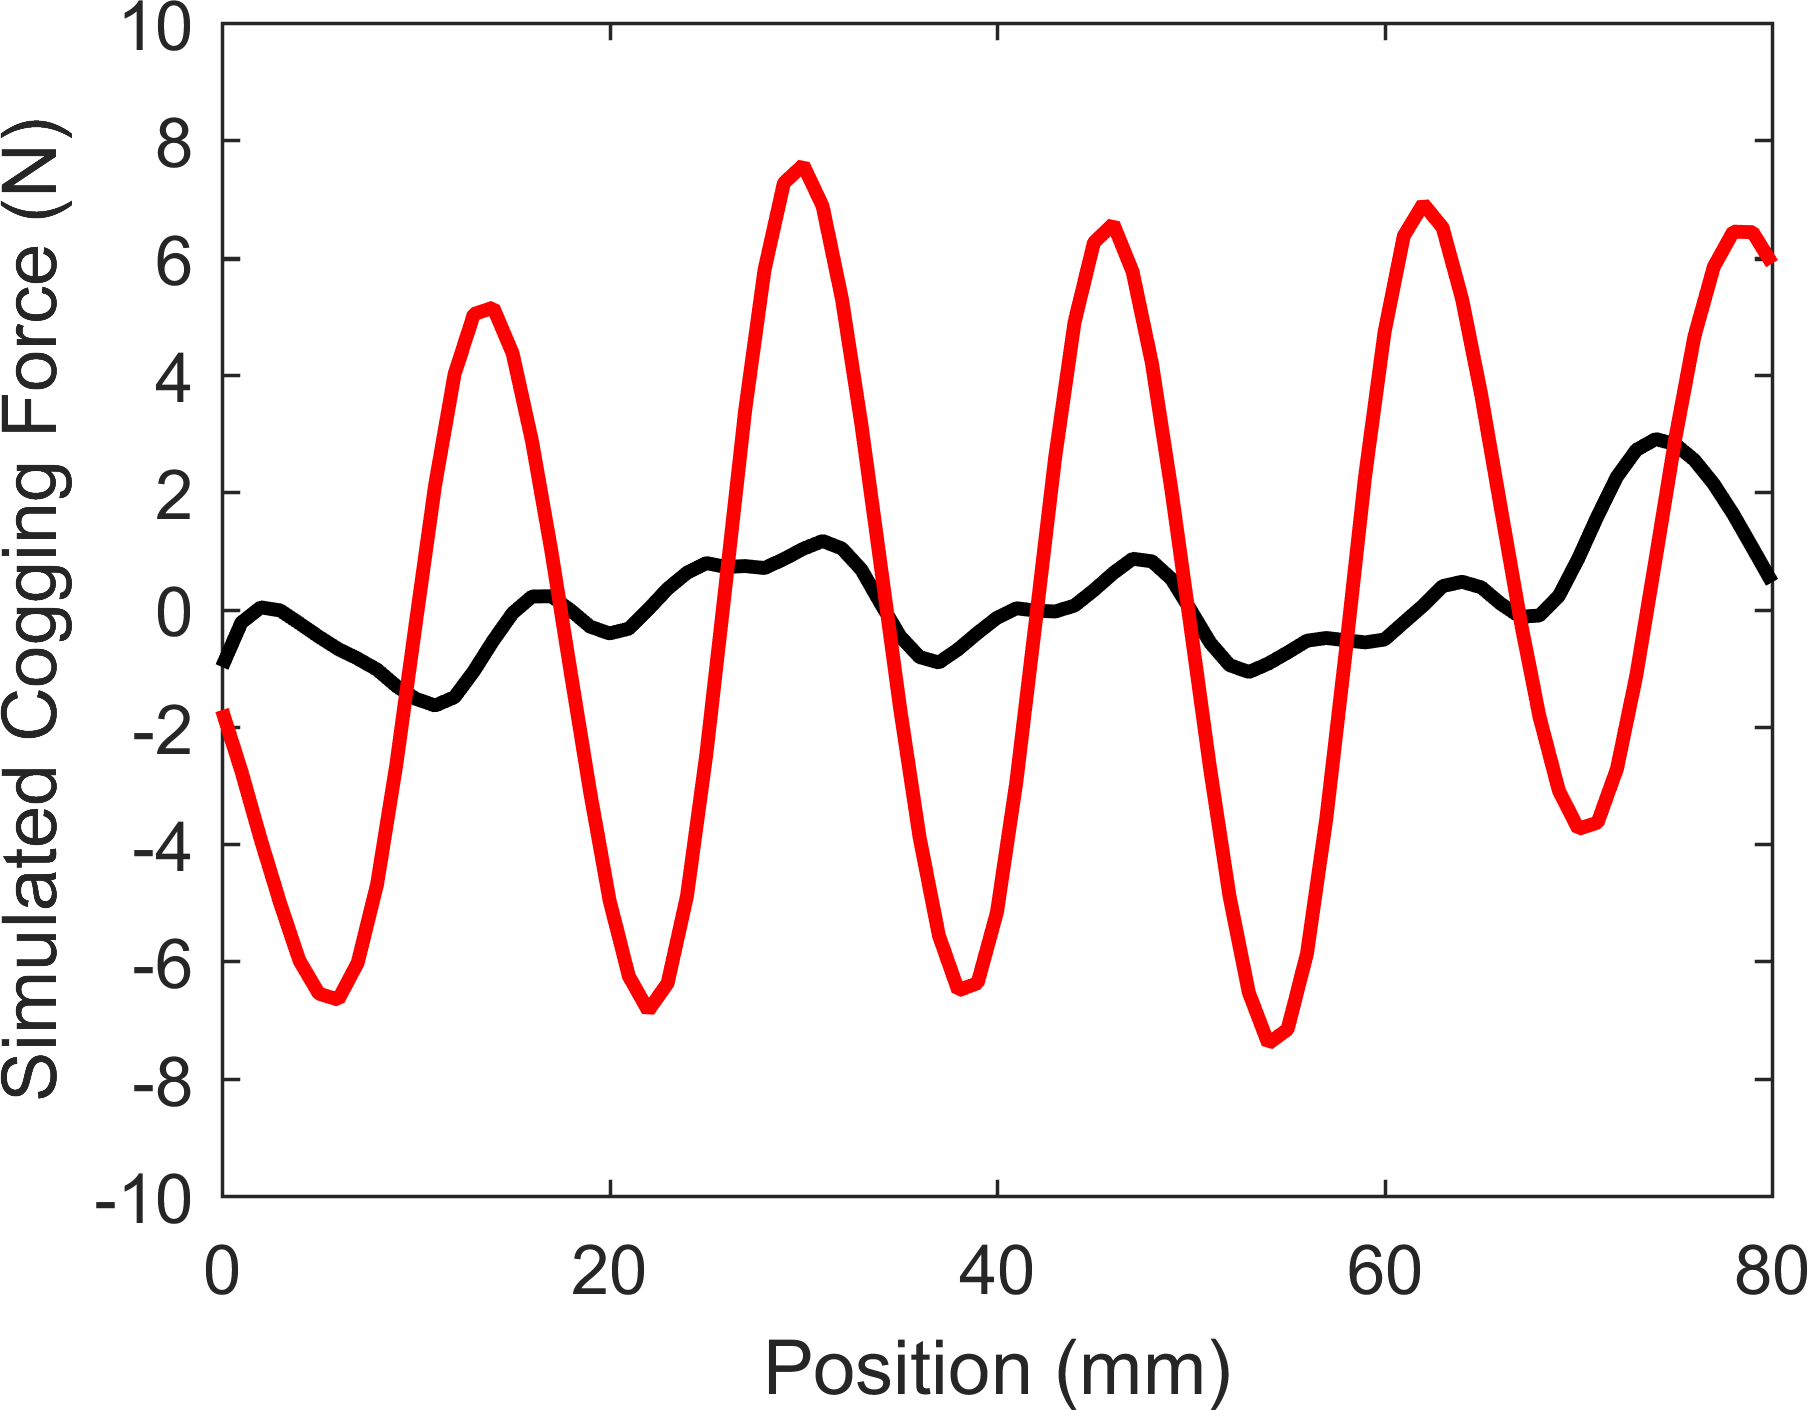
\includegraphics[width=3.45in]{chap5/images/Compare_cogging_FEA.png}
            \label{fig:chap/experiment/cogging/Compare_cogging_FEA}
        }
        \caption{Peak to peak cogging force $Max(F_C) - Min(F_C )$ against iron length $\lambda = 64 \rightarrow 96 \,\mathrm{mm}$, using the globally optimized motor configuration, with each point collected by moving back-iron over the entire stroke length $L_s$ in (a); and comparison between the cogging force distributions of the worst-case iron length $L_f = 79\,\mathrm{mm}$\,(black) and the chosen $L_f = 71\,\mathrm{mm}$\,(red) in (b).}
    \end{figure}
    

    The chosen motor configuration consists of four half-coil-poles with the minimum back-iron length $L_f = 64\,\mathrm{mm}$. The automation script swept for extra back-iron lengths of $\lambda = 0 \rightarrow 32\,\mathrm{mm}$, with increment of $\operatorname d\lambda = 0.5\,\mathrm{mm}$, over the entire stroke length of $\Delta = 0 \rightarrow 80\,\mathrm{mm}$, with increment of $\operatorname d\Delta = 0.5\,\mathrm{mm}$. We chose the back-iron tube length to be $L_f = 71\,\mathrm{mm}$ for having the least peak to peak cogging force $\operatorname{Max}(F_C) - \operatorname{Min}(F_C ) = 4.07\,\mathrm{N}$. The chosen back-iron length of $L_f = 71\,\mathrm{mm}$ reduces cogging force $71.5\,\%$ compared to the minimal choice of $L_f = L_C = 64\,\mathrm{mm}$, as shown in  Fig.~\ref{fig:chap/experiment/cogging/Cogging_sweep_FEA}. With a maximum FEA axis-xymmetric grid size of $0.5\,\mathrm{mm}$, the whole process took $14$\,hours on an Intel i7 - 4970 CPU.


% ===================================================================================================
% === NEW SECTION === NEW SECTION === NEW SECTION === NEW SECTION === NEW SECTION === NEW SECTION ===
% ===================================================================================================
\section{Validation}                                \label{Chapter:experiment/validation}


        % -----------------------------------------------------------------------------------
        % --- NEW SUB SECTION --- NEW SUB SECTION --- NEW SUB SECTION --- NEW SUB SECTION --- 
        % -----------------------------------------------------------------------------------
        \subsection{Construction}                   \label{Chapter:construction}
        
        
            \begin{figure}[h]
                \centering
                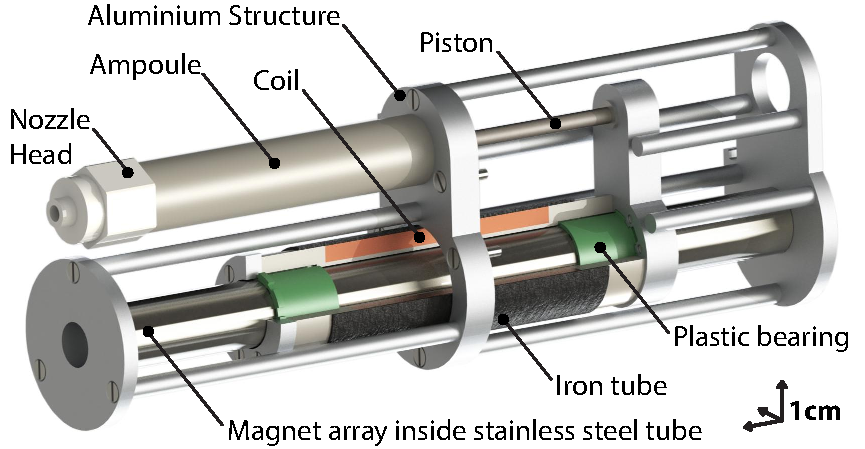
\includegraphics[width=5in]{chap5/images/PMLSM_render.pdf}
                \caption{Cut-away view of the optimized motor and jet injector design, showing the bobbin and coil riding on linear plastic bearings along the magnet array, as well as the supporting structure, piston, and drug ampoule.}
                \label{fig:chap/experiment/PMLSM render}
            \end{figure}
                
        
            Based upon the results of these optimizations obtained summarized in Table\,\ref{table:chap/validation/construction/final_motor_design_params}, we constructed a prototype motor and jet injector structure as shown in Fig.\,\ref{fig:chap/experiment/validation/construction/overall_construction}. In this prototype, each phase coil was wound using $180$ turns of $28.5\,\mathrm{AWG}$ wire; four coils were joined in series to form each phase, with a phase resistance of $11.6\,\Omega$. The back-iron was provided with a $2\,\mathrm{mm}$ slit to facilitate electrical connection; narrow slits of this sort have been shown to have negligible effect on motor performance, and may have advantageous effects in reducing eddy currents\,\cite{Meessen2009}. Fig.\,\ref{fig:chap/experiment/PMLSM render} shows a render of the mechanical design concept for the prototype \acs{PMLSM} with the optimized dimensions. In this initial prototype, a back-iron length of $79\,\mathrm{mm}$ was chosen, so as to explore the properties of a high-cogging-force regime, as well as the optimal length of $71\,\mathrm{mm}$.
        
        
            \begin{table}[h]
            \renewcommand{\arraystretch}{1.2}
            \caption{Summary of motor design values}
            \label{table:chap/validation/construction/final_motor_design_params}
            \centering
                \begin{tabular}{llr}
                \hline
                \bfseries Parameter & \bfseries Description & \bfseries Values\\
                \hline
                    $N_M$			& Number of half magnet-poles			&	$9$\\
                    $N_C$			& Number of half coil-poles				&	$4$\\
                    $r_{mi}$		& Magnet array inner radius 			&	$2\,\mathrm{mm}$\\ 
                    $r_{mo}$		& Magnet array outer radius  			&	$7.8\,\mathrm{mm}$\\
                    $r_{ci}$		& Coil array inner radius				&	$9.1\,\mathrm{mm}$\\ 
                    $r_{co}$		& Coil array outer radius 				&	$13.1\,\mathrm{mm}$\\ 
                    $r_{fi}$		& Iron tube inner radius 				&	$13.2\,\mathrm{mm}$\\ 
                    $r_{fo}$		& Iron tube outer radius	 			&	$13.93\,\mathrm{mm}$\\ 
                    $\delta$		& Ratio of radial magnet vs. magnet pair	&	$0.258$\\ 
                \hline
                	$L_k$ 			& Repeat length 							&	$64\,\mathrm{mm}$\\
                	$L_M$			& Magnet array total length				&	$144\,\mathrm{mm}$\\ 
                	$L_C$			& Coil array total length				&	$64\,\mathrm{mm}$\\ 
                	$L_f$			& Iron tube length						&	$71\,\mathrm{mm}$\\ 
                    $L_s$			& Stroke length 						&	$80\,\mathrm{mm}$\\
                \hline
                \end{tabular}
            \end{table}
            
            
            \begin{figure}[h]
            \centering
            \subfloat[The bobbin with fully wound coil (left) \& iron tube assembly (right)]{
                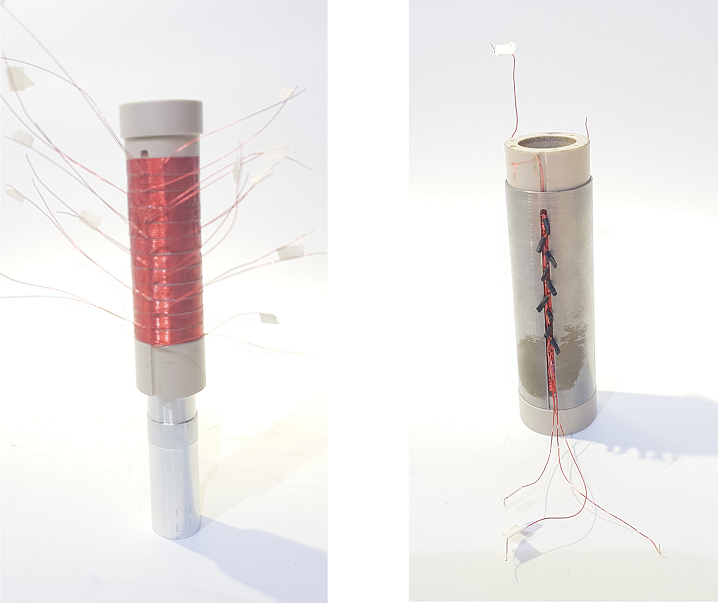
\includegraphics[width=4.3in]{chap5/images/winding_completed.png}
                \label{fig:chap/experiment/validation/construction/winding_completed}
            }
            \\
            \subfloat[Full motor assembly without the ampoule]{
                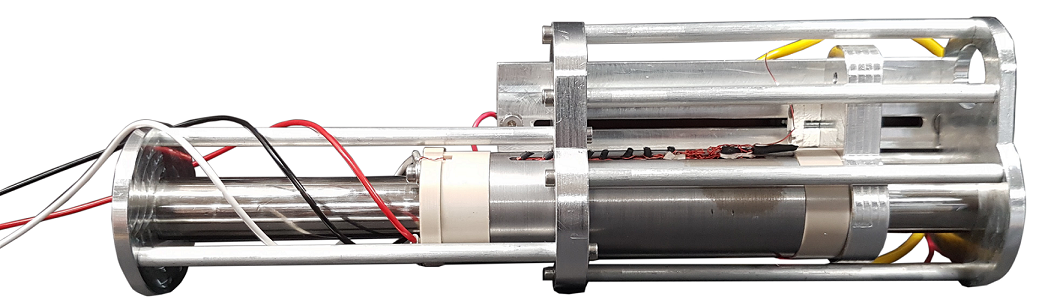
\includegraphics[width=5.4in]{chap5/images/assemnly_without_ampoule.png}
                \label{fig:chap/experiment/validation/construction/assemnly_without_ampoule}
            }
            \caption{Pictures showing progress of the device construction: the bobbin with a fully wound coil, as well as the bobbin with coil and iron tube assembly\,(a); and the full motor assembly without the NFJI ampoule and casing\,(b).}
            \label{fig:chap/experiment/validation/construction/overall_construction}
            \end{figure}
            
            
            The magnets (Grade $\mathrm{N45SH}$, K\&J Magnetics) were assembled inside a stainless steel tube ($16\,\mathrm{mm}$ outside diameter), with the radial magnets provided as four uniformly-magnetized segments. In addition to containing the repulsive forces acting upon the radial magnet segments, this tube also served as a bearing surface for polymer sleeve bearings integrated into the ends of the bobbin.
    
    
            The motor was integrated into an injector structure parallel and adjacent to the drug ampoule, yielding a compact arrangement. This configuration requires the motor bearings and connecting structures to resist a moment, requiring the widely-spaced bearings and the use of a thick force-transmitting plate between the piston and the coil. A linear potentiometer (Bourns PTB) was used for absolute motor position measurement. As shown in Fig.\,\ref{fig:chap/experiment/validation/construction/assemnly_without_ampoule}, the motor and structure have a mass of $605\,\mathrm{g}$.
    

        % -----------------------------------------------------------------------------------
        % --- NEW SUB SECTION --- NEW SUB SECTION --- NEW SUB SECTION --- NEW SUB SECTION ---
        % -----------------------------------------------------------------------------------
        \subsection{Motor constant measurement}     \label{Chapter:experiment/validation/motor constant}
        
            
            The motor constant was evaluated by measurement of the phase back-EMF during the externally-induced motion was applied on the armature mover. The phase voltage constant measurements for each of the three phases are plotted on Fig.~\ref{fig:chap/experiment/motor_constant/kms_plot}, with the phases connected in a wye topology. A load cell (Futek LCM300, $250\,\mathrm{lb.}$ capacity) was used to simultaneously determine the cogging force exhibited by the prototype. 

        
            \begin{figure}[h]
                \centering
                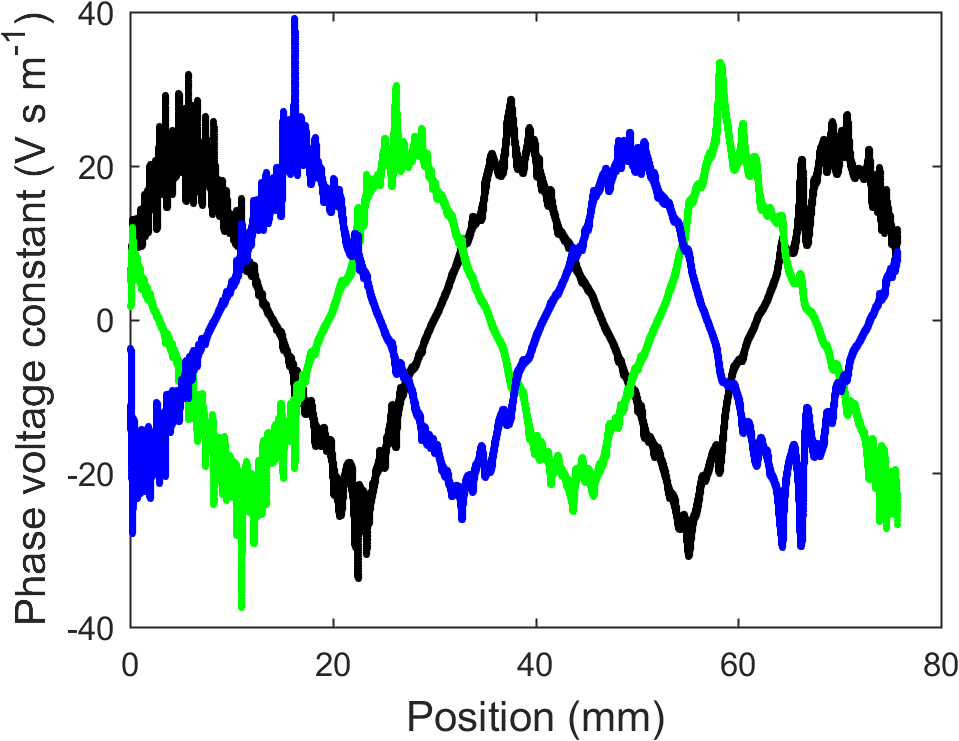
\includegraphics[width=3.4in]{chap5/images/kms_plot.png}
                \caption{Measured phase voltage constant $K_e$ against motor position for each motor phase, determined over multiple passes at different velocities between $10\,\mathrm{mm/s}$ and $25\,\mathrm{mm/s}$. There is a range in velocity because the coil was moved by hand.}
                \label{fig:chap/experiment/motor_constant/kms_plot}
            \end{figure}


            The measured voltage constants for the three phases are shown in Fig.~\ref{fig:chap/experiment/motor_constant/kms_plot}. The relatively narrow radial magnets and close proximity of iron yield a triangular flux waveform, with minimal end effects; noise near the peaks is likely a result of the relatively slow movement velocity employed ($\sim0.1\,\mathrm{m/s}$). 
            
            Based upon these voltage constants and the phase resistance, the motor constant is $6.6\,\mathrm{N/ \sqrt{ \mathrm{W}}}$, within $10\,\%$ of the design value of $7.2\,\mathrm{N/ \sqrt{ \mathrm{W}}}$. This would correspond to an operating power of $1.4\,\mathrm{kW}$, rather than the design point of $1.2\,\mathrm{kW}$. The reduced performance seen in the prototype appears to be due largely to a reduced winding fill factor from that which was expected, and may be improved by improved winding and interconnection technique.

        
        
        % -----------------------------------------------------------------------------------
        % --- NEW SUB SECTION --- NEW SUB SECTION --- NEW SUB SECTION --- NEW SUB SECTION ---
        % -----------------------------------------------------------------------------------
        \subsection{Cogging force measurement}      \label{Chapter:experiment/validation/cogging force}
        
        
            The measured cogging force is shown in Fig.\,\ref{fig:chap/experiment/validation/cogging_force/cogging_measurement}, after correcting for bearing friction of $4.2\,\mathrm{N}$. The peak-to-peak amplitude for the $79\,\mathrm{mm}$ back-iron is approximately $14\,\mathrm{N}$, and for the $71\,\mathrm{mm}$ back-iron is $4\,\mathrm{N}$, in close agreement with the predictions shown in Fig.\,\ref{fig:chap/experiment/cogging/Compare_cogging_FEA}. There is also good agreement in the details of the cogging force waveform, with slight differences near one end of the stroke.
            
            
            \begin{figure}[h]
                \centering
                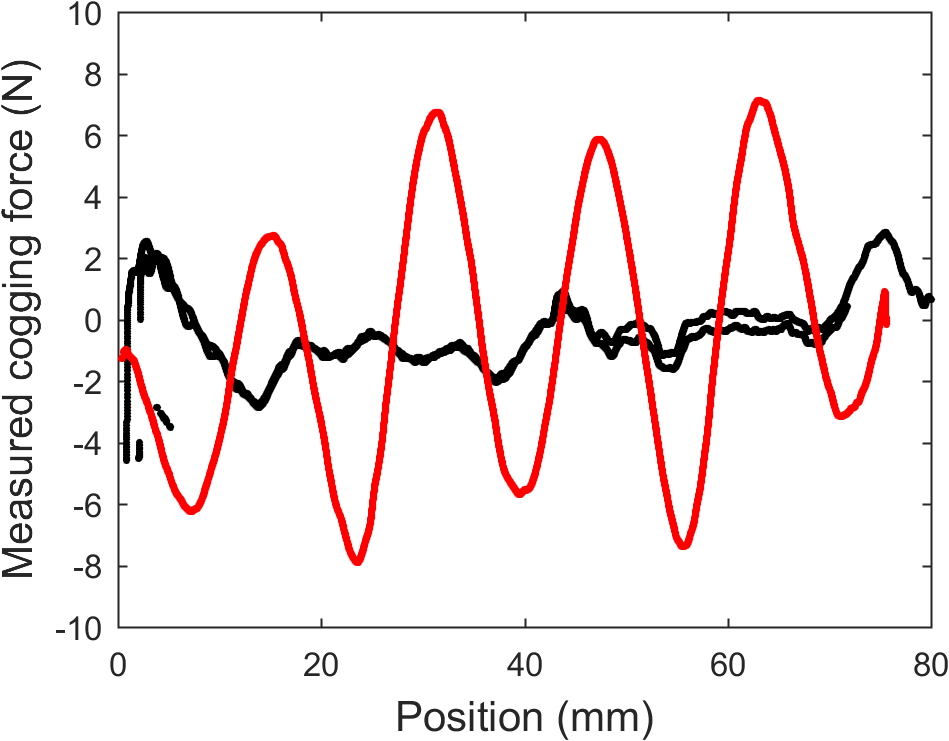
\includegraphics[width=3.4in]{chap5/images/cogging_measurement.png}
                \caption{Measured cogging force due to finite back-iron length, for a back-iron length of $79\,\mathrm{mm}$ (red) and a length of $71\,\mathrm{mm}$ (black). Position is measured relative to one end of the motor stroke.}
                \label{fig:chap/experiment/validation/cogging_force/cogging_measurement}
            \end{figure}
        
        
        % -----------------------------------------------------------------------------------
        % --- NEW SUB SECTION --- NEW SUB SECTION --- NEW SUB SECTION --- NEW SUB SECTION ---
        % -----------------------------------------------------------------------------------
        \subsection{Injection test in air}              \label{Chapter:experiment/validation/injection test}
        
        
            The other key component in a practical injection system is the power electronic drive, which needs to provide a burst of high power for a short time from a compact package. We have recently reported on such a system designed for a voice coil actuator\,\cite{Ruddy2017}. The newest iteration of the device was built to be capable of three-phase drive to control the prototype motor for NFJI.


            \begin{figure}[h]
                \centering
                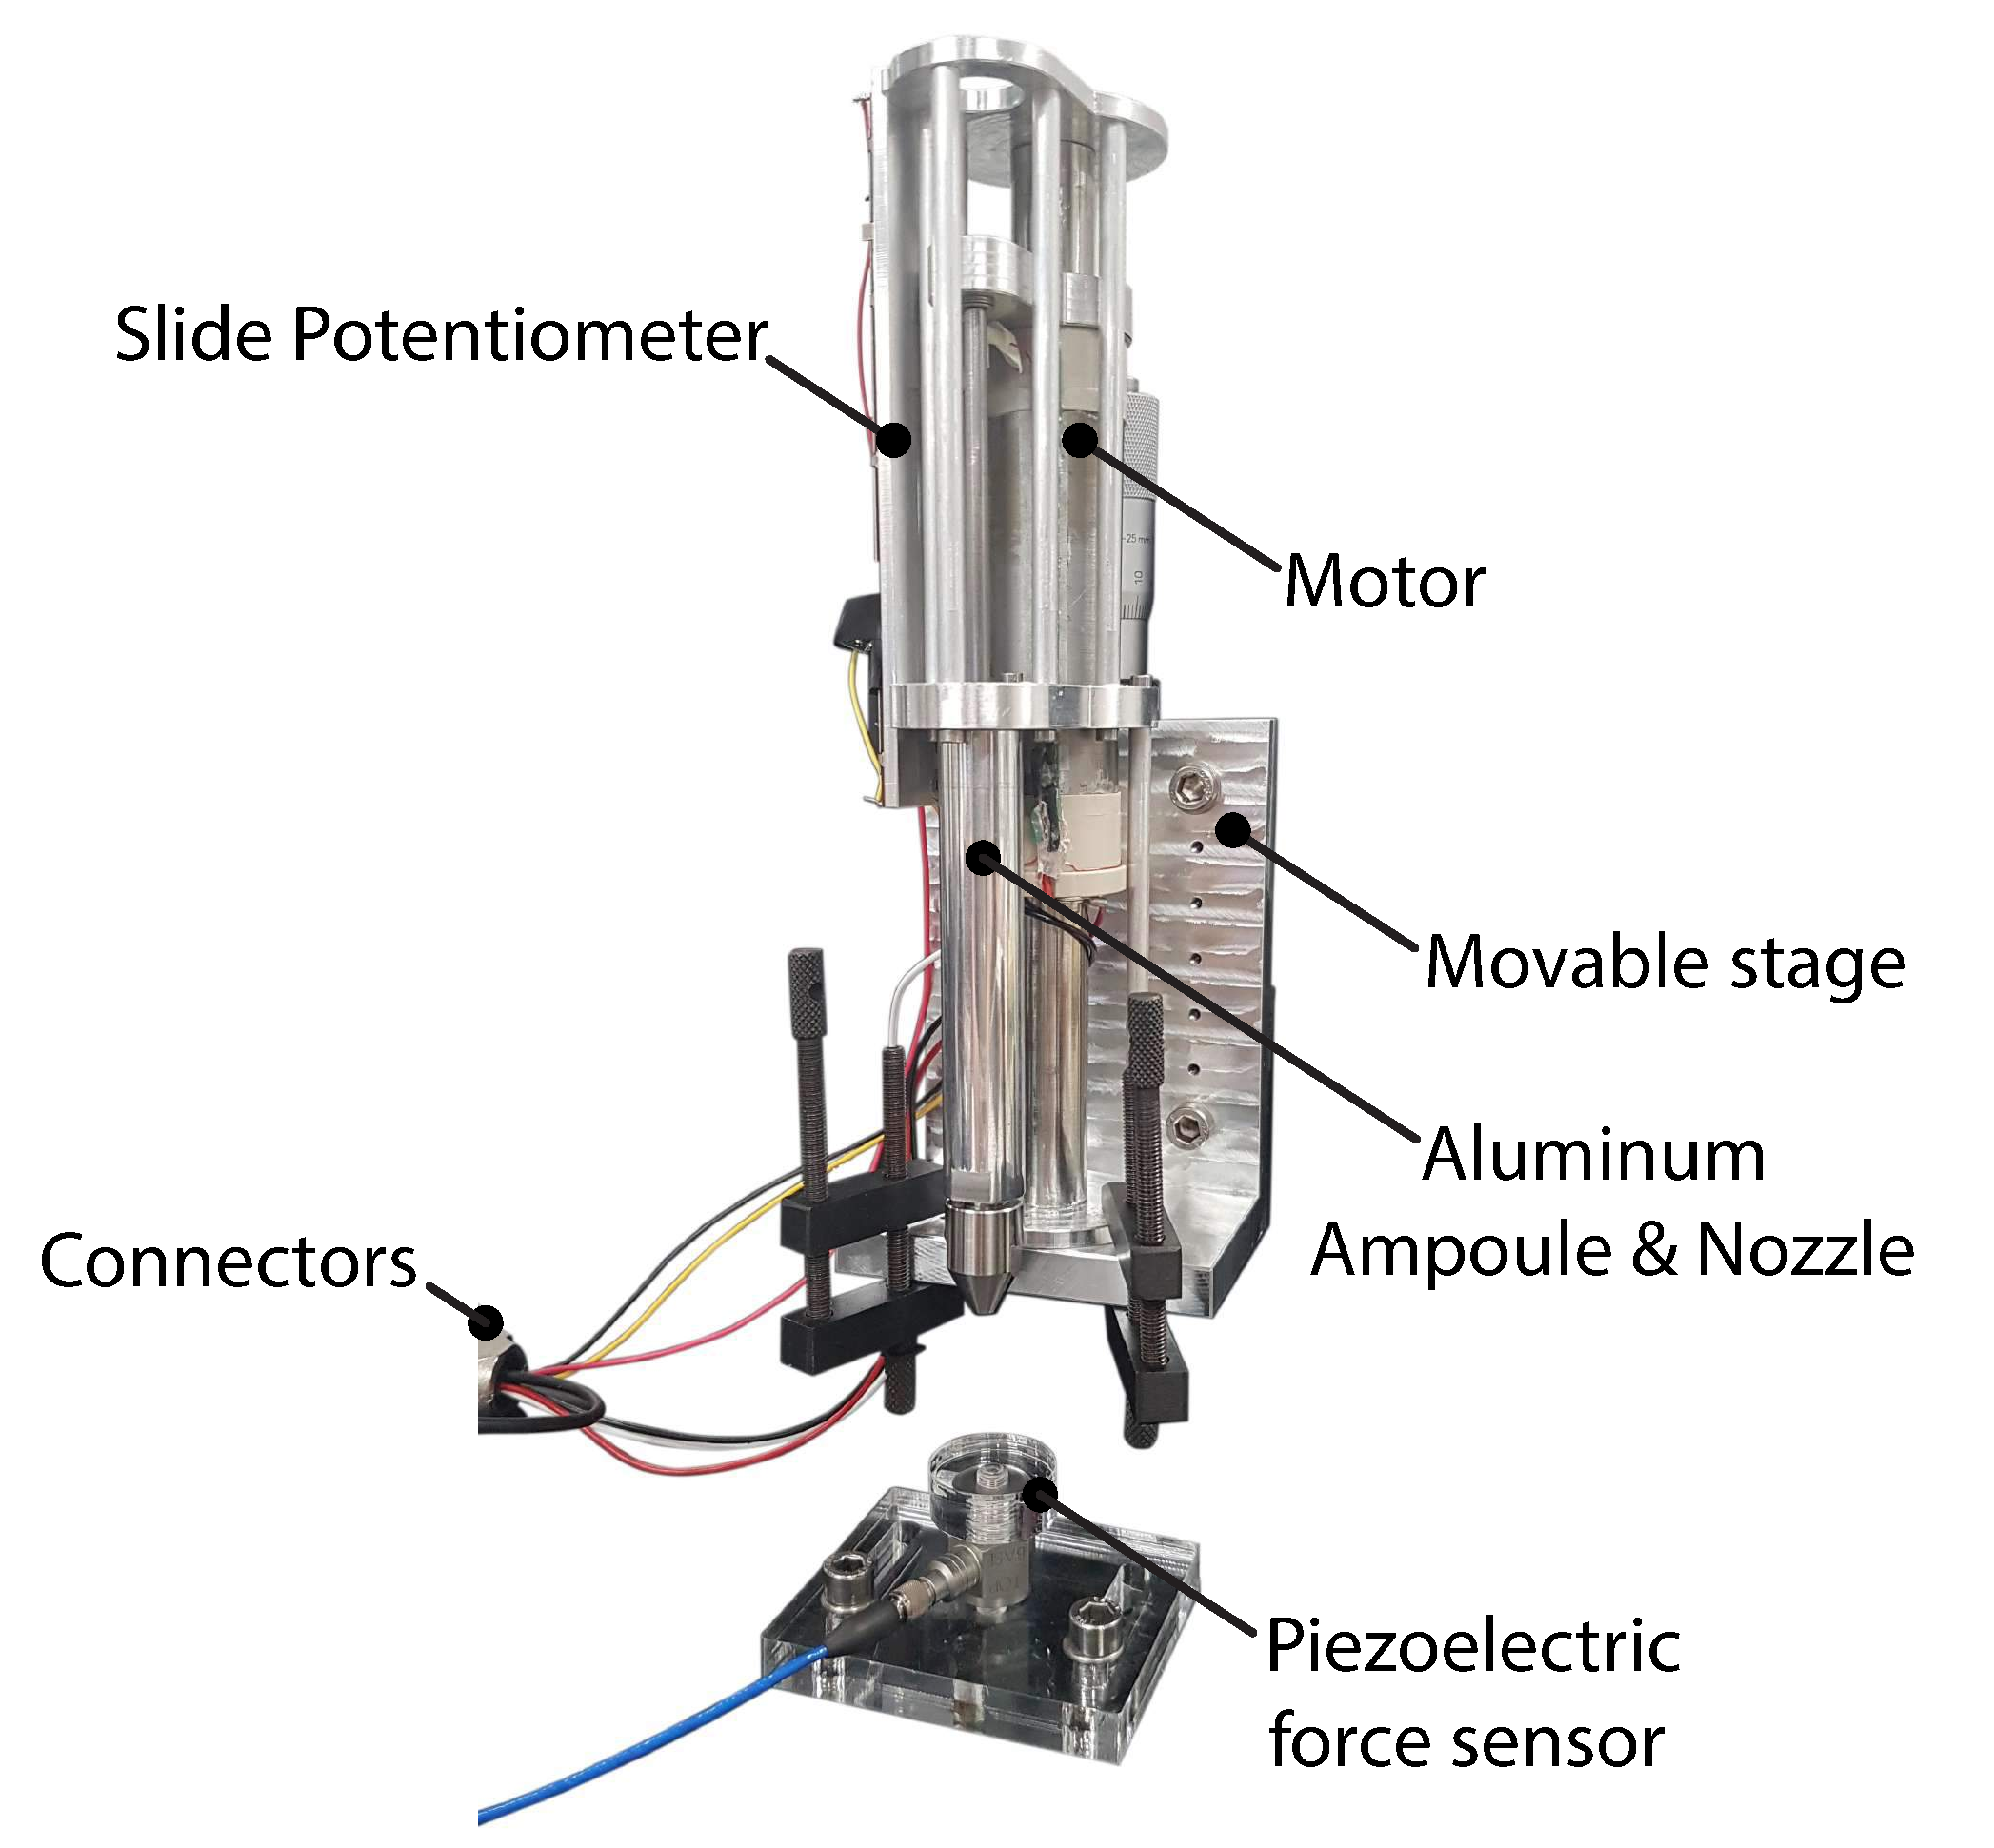
\includegraphics[width=4in]{chap5/images/injection_setup.pdf}
                \caption{Experimental setup in which the motor ejects water onto a piezoelectric force sensor, driven with constant motor input voltage}
                \label{fig:chap/experiment/validation/injection_test/injection_setup}
            \end{figure}


            To validate the practical performance of the motor in performing needle-free jet injections, we inserted into it an ampoule and orifice, and estimated the velocity of the jet produced by directing it against a piezoelectric force sensor (model $208\mathrm{C}01$, PCB Piezotronics). By measuring the jet velocity in this way, we eliminate any potential effects from leakage or fluid compression. In Fig.~\ref{fig:chap/experiment/validation/injection_test/injection_setup}, the experimental setup comprises the fully assembled motor mounted on a movable stage, with an aluminum ampoule filled with water pointing at the force sensor, and the power system to drive the motor (not shown here). Fig.~\ref{fig:chap/experiment/injection_test/injection_test} shows the results for a water jet ejection onto the force sensor placed $15\,\mathrm{mm}$ away from the tip of the nozzle. The controller applied a constant phase voltage amplitude of $110\,\mathrm{V_{rms}}$, corresponding to a nominal power of $1.4\,\mathrm{kW}$, for a period of $0.1\,\mathrm{s}$. Based on the measured travel distance of the motor piston, as shown in Fig.~\ref{fig:chap/experiment/injection_test/position_waveform}, the average jet speed achieved was $134\,\mathrm{m/s}$. This value is obtained from the relationship between the piston tip velocity $v_{piston}$ and the water jet velocity $v_{jet}$, assuming an incompressible fluid and uniform plug flow:
            
            \begin{equation}
            v_{jet}=v_{piston} \frac{A_{piston}}{A_{jet}}
            \label{eq:chap/validation/injection_test/v_jet estimated from area}
            \end{equation}
            
            where $A_{piston}$, and $A_{jet}$ are the cross sectional area of the piston, and jet nozzle, in the same order. Furthermore, the instantaneous force\,$F_{ins}$ measured by the piezoelectic force sensor can be also translated to jet velocity\,$v_{jet}$, given $A_{jet}$, and known density of water $\rho_{water}$, assuming a uniform plug flow: 
            
            \begin{equation}
            v_{jet}=\sqrt{\frac{F_{ins}}{\rho_{water}A_{jet}}}
            \label{eq:chap/validation/injection_test/v_jet estimated from force}
            \end{equation}
            
            The average jet speed calculated from the force measurement was slightly higher than the jet speed estimated by the position profile, at $144\,\mathrm{m/s}$. This is likely because the flow exiting the nozzle does not have a uniform velocity profile, which tends to increase the apparent jet speed obtained via force measurement. These jet speeds are well within the range of speeds useful in jet injection, and in line with other jet speeds obtained with this nominal pressure \cite{Williams2016}.


            \begin{figure}[h]
            	\centering
            	\subfloat[Measured motor position]{
            		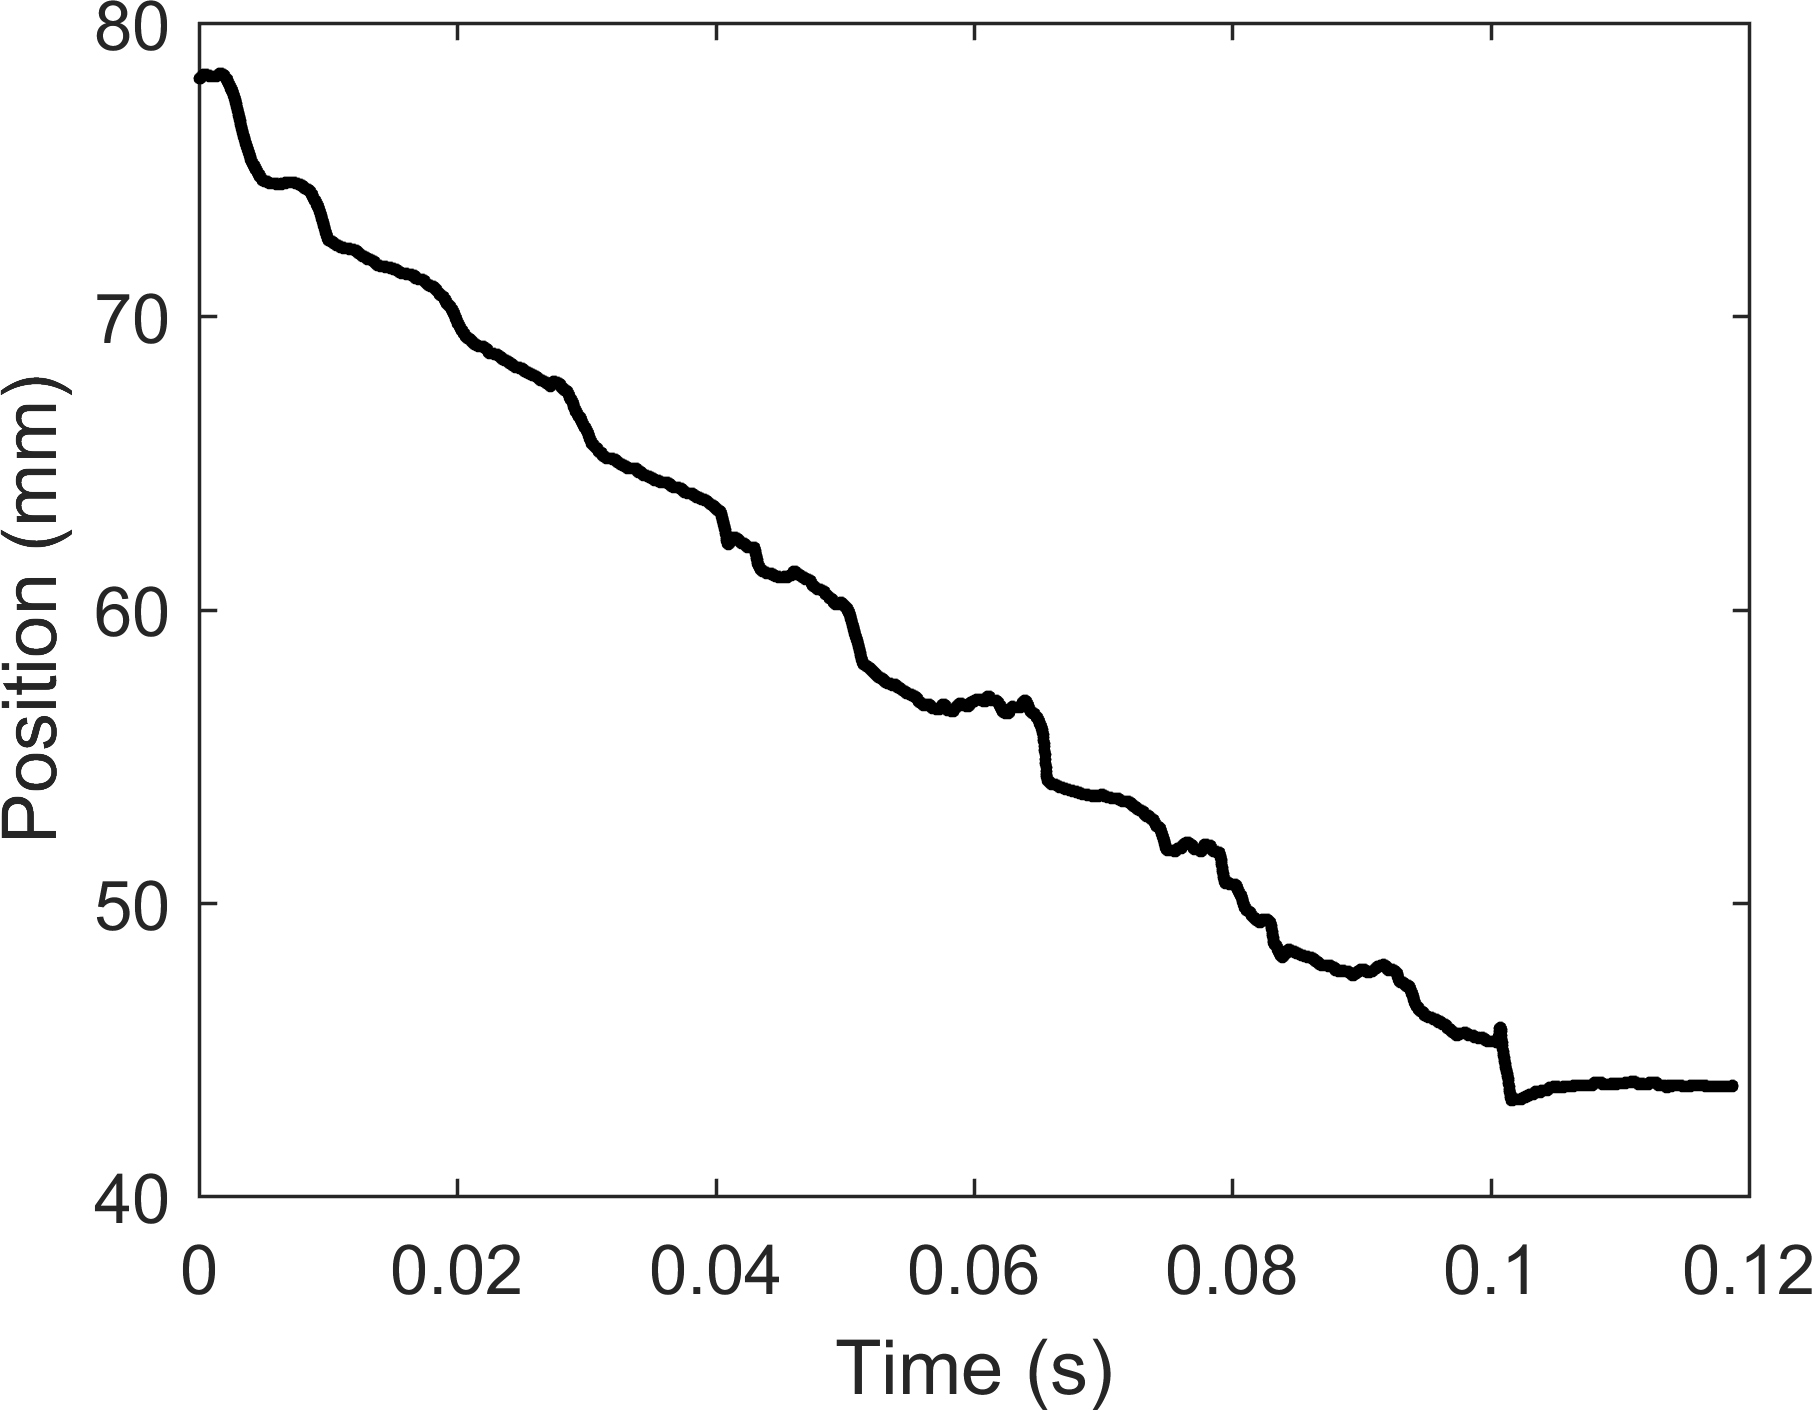
\includegraphics[width=2.75in]{chap5/images/position_waveform.png}
            		\label{fig:chap/experiment/injection_test/position_waveform}
            	}
            	\,\,
            	\subfloat[Jet velocity determined from force measurement]{
            		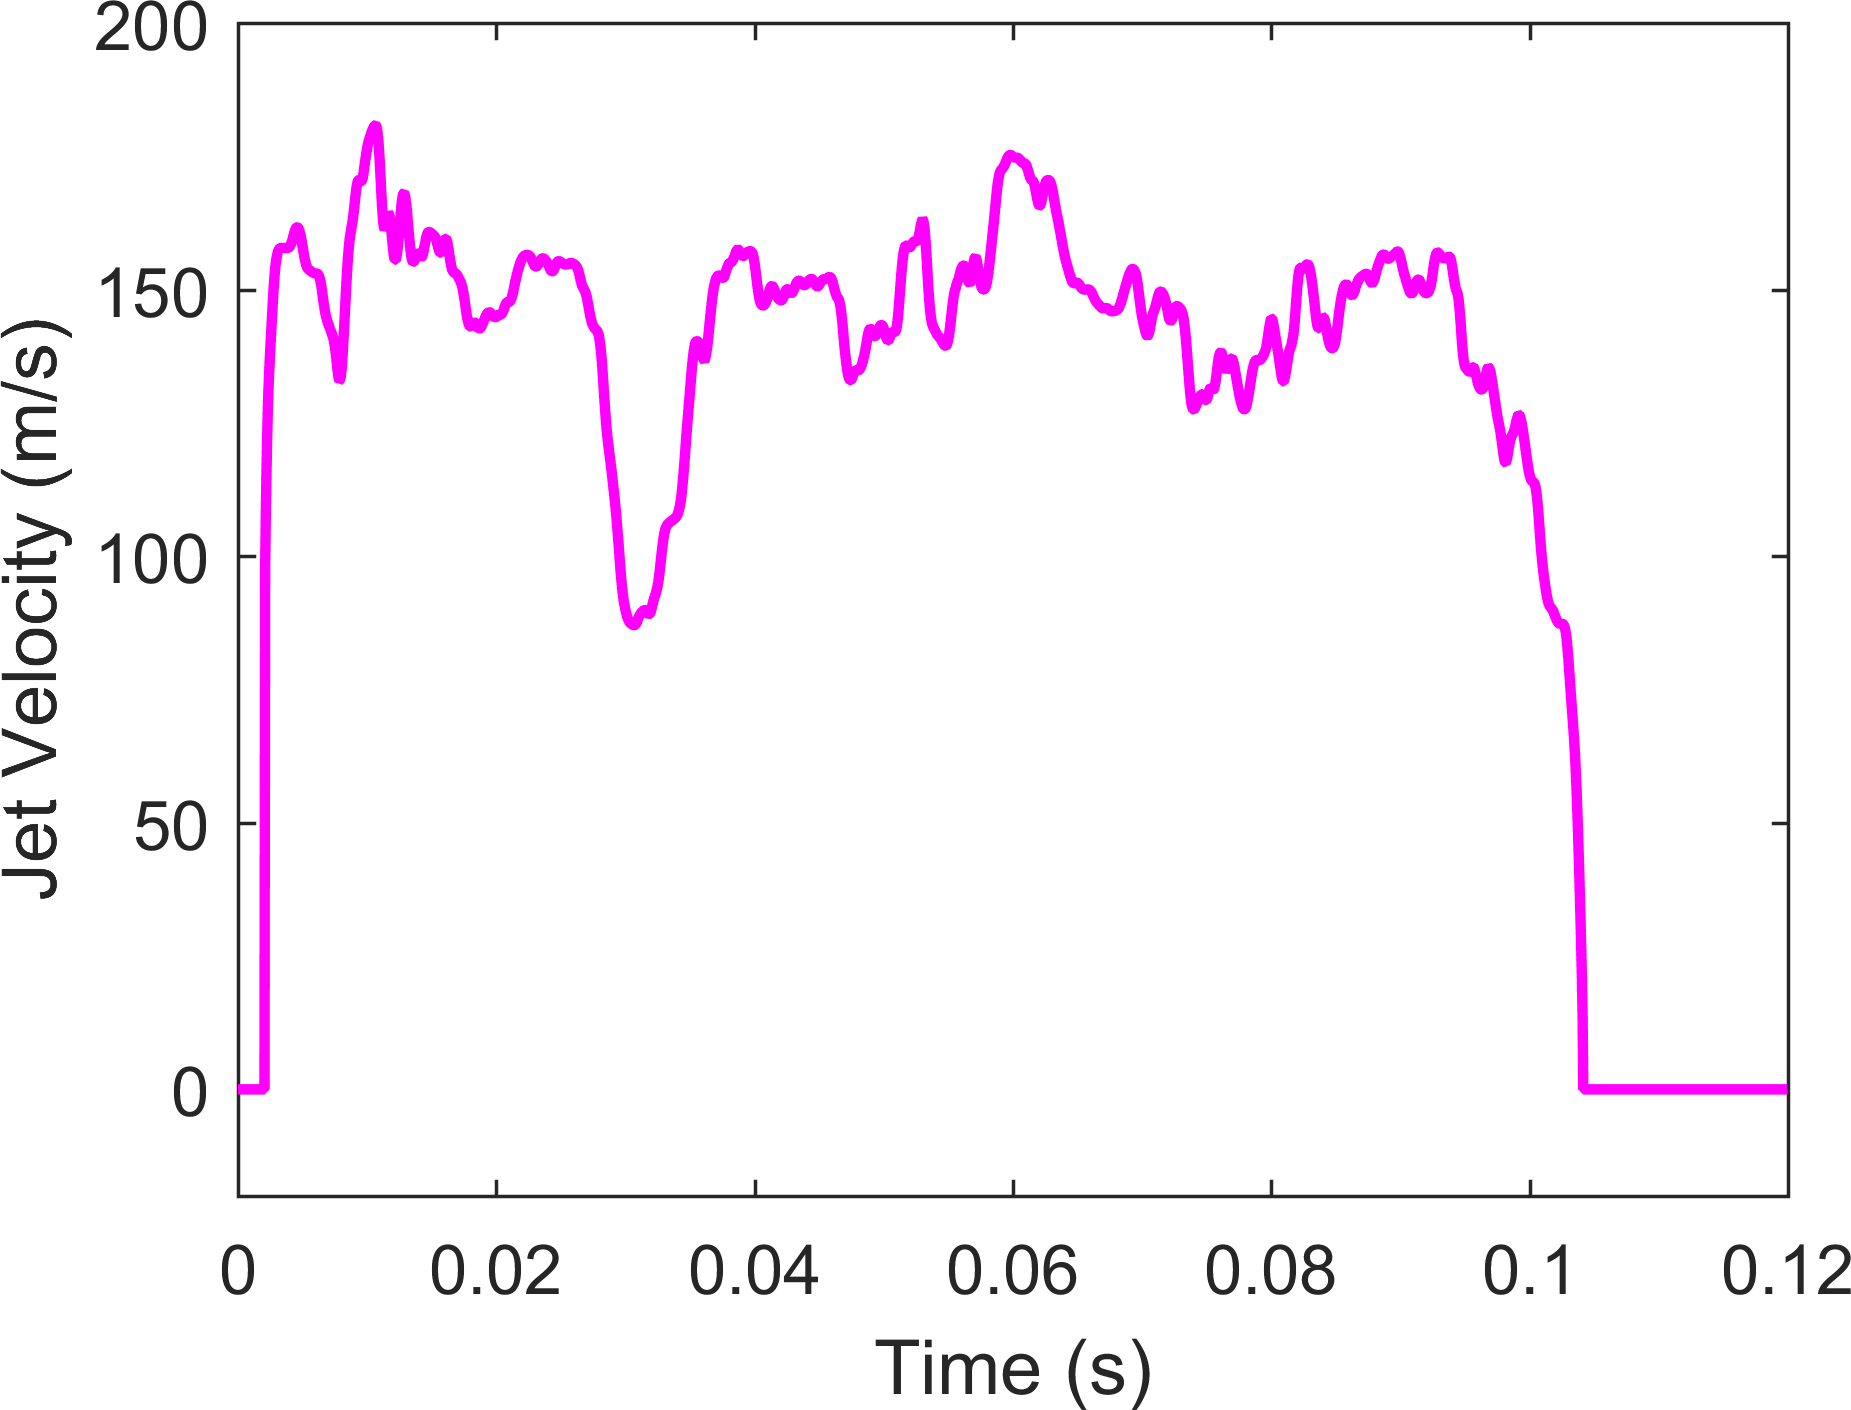
\includegraphics[width=2.75in]{chap5/images/velocity_waveform.png}
            		\label{fig:chap/experiment/injection_test/velocity_waveform}
            	}
            	\\
                \subfloat[Three-phase current during the injection]{
            		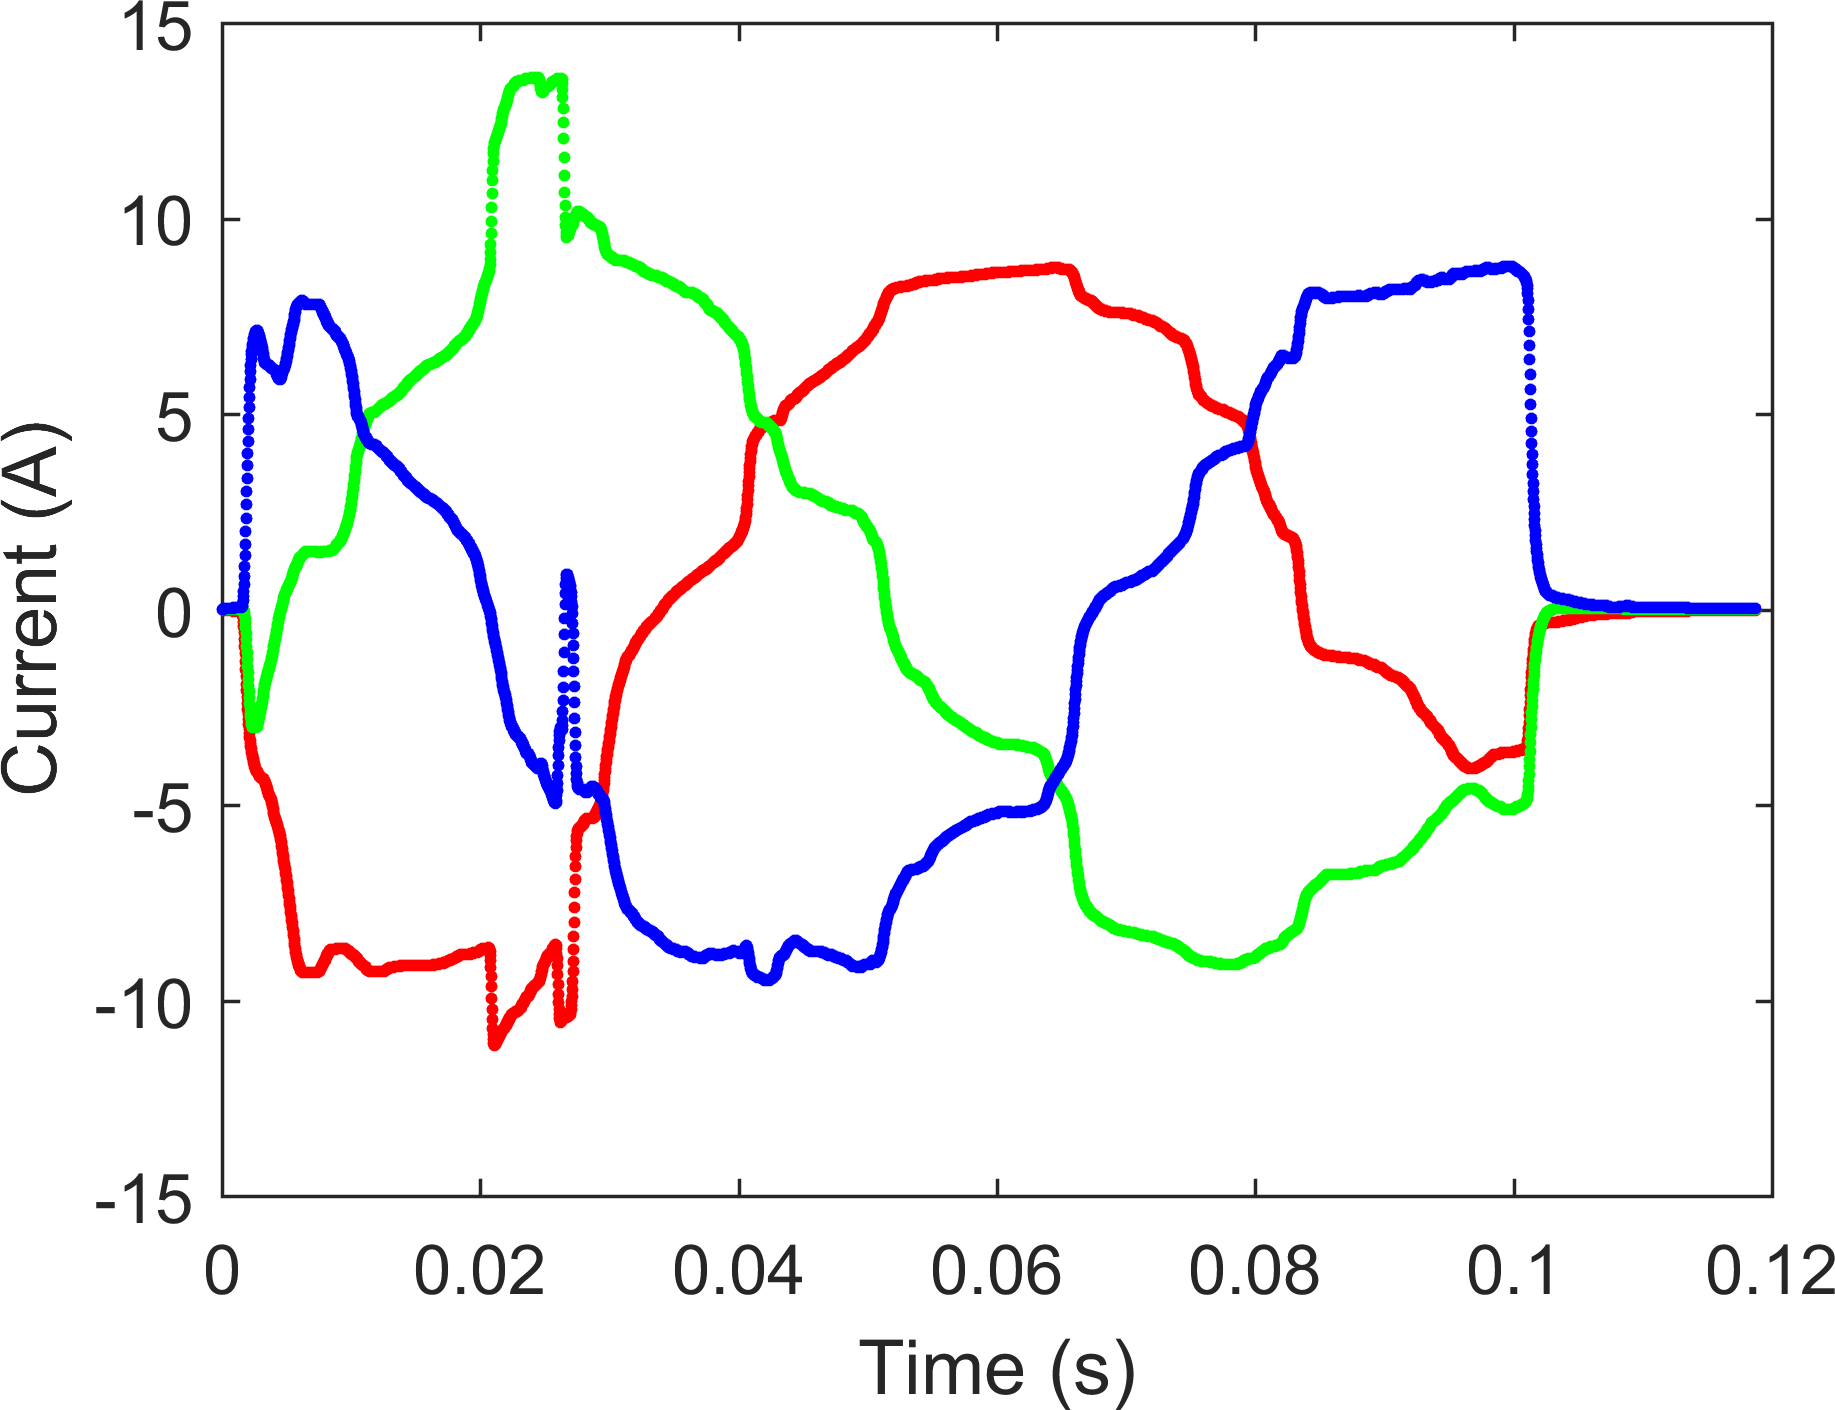
\includegraphics[width=2.8in]{chap5/images/current_waveform.png}
            		\label{fig:chap/experiment/injection_test/current_waveform}
            	}
                \caption{Measured piston position for a constant-voltage injection corresponding to a nominal power of $1.4\mathrm{kW}$ (a); the jet velocity determined from the force of the water jet acting upon the force sensor (b); and the current profile across the motor phases during the injection (c).}
                \label{fig:chap/experiment/injection_test/injection_test}
            \end{figure}


            Despite the use of an open-loop, constant-voltage-amplitude control approach, the jet speed was relatively steady throughout the stroke, and most variations observed correspond to changes in the friction and cogging forces. The dip in velocity near the beginning of the injection may be due to the fact that during the loading process, an air bubble made its way into the ampoule. When the bubble approaches the output nozzle, the lack of fluid can cause sudden changes in velocity. Air bubbles can only be avoided through careful filling procedures.
            
            
            These results validate that the prototype motor is capable delivering large volume needle free jet injection (up to $1\,\mathrm{mL}$) when given $1.4\,\mathrm{kW}$ of electrical power, close to the theoretical design value of $1.2\,\mathrm{kW}$. Improvements to the motor control strategy will allow for further enhancements to injection consistency and repeatability.
            
    
            \begin{figure}[h]
            	\centering
            	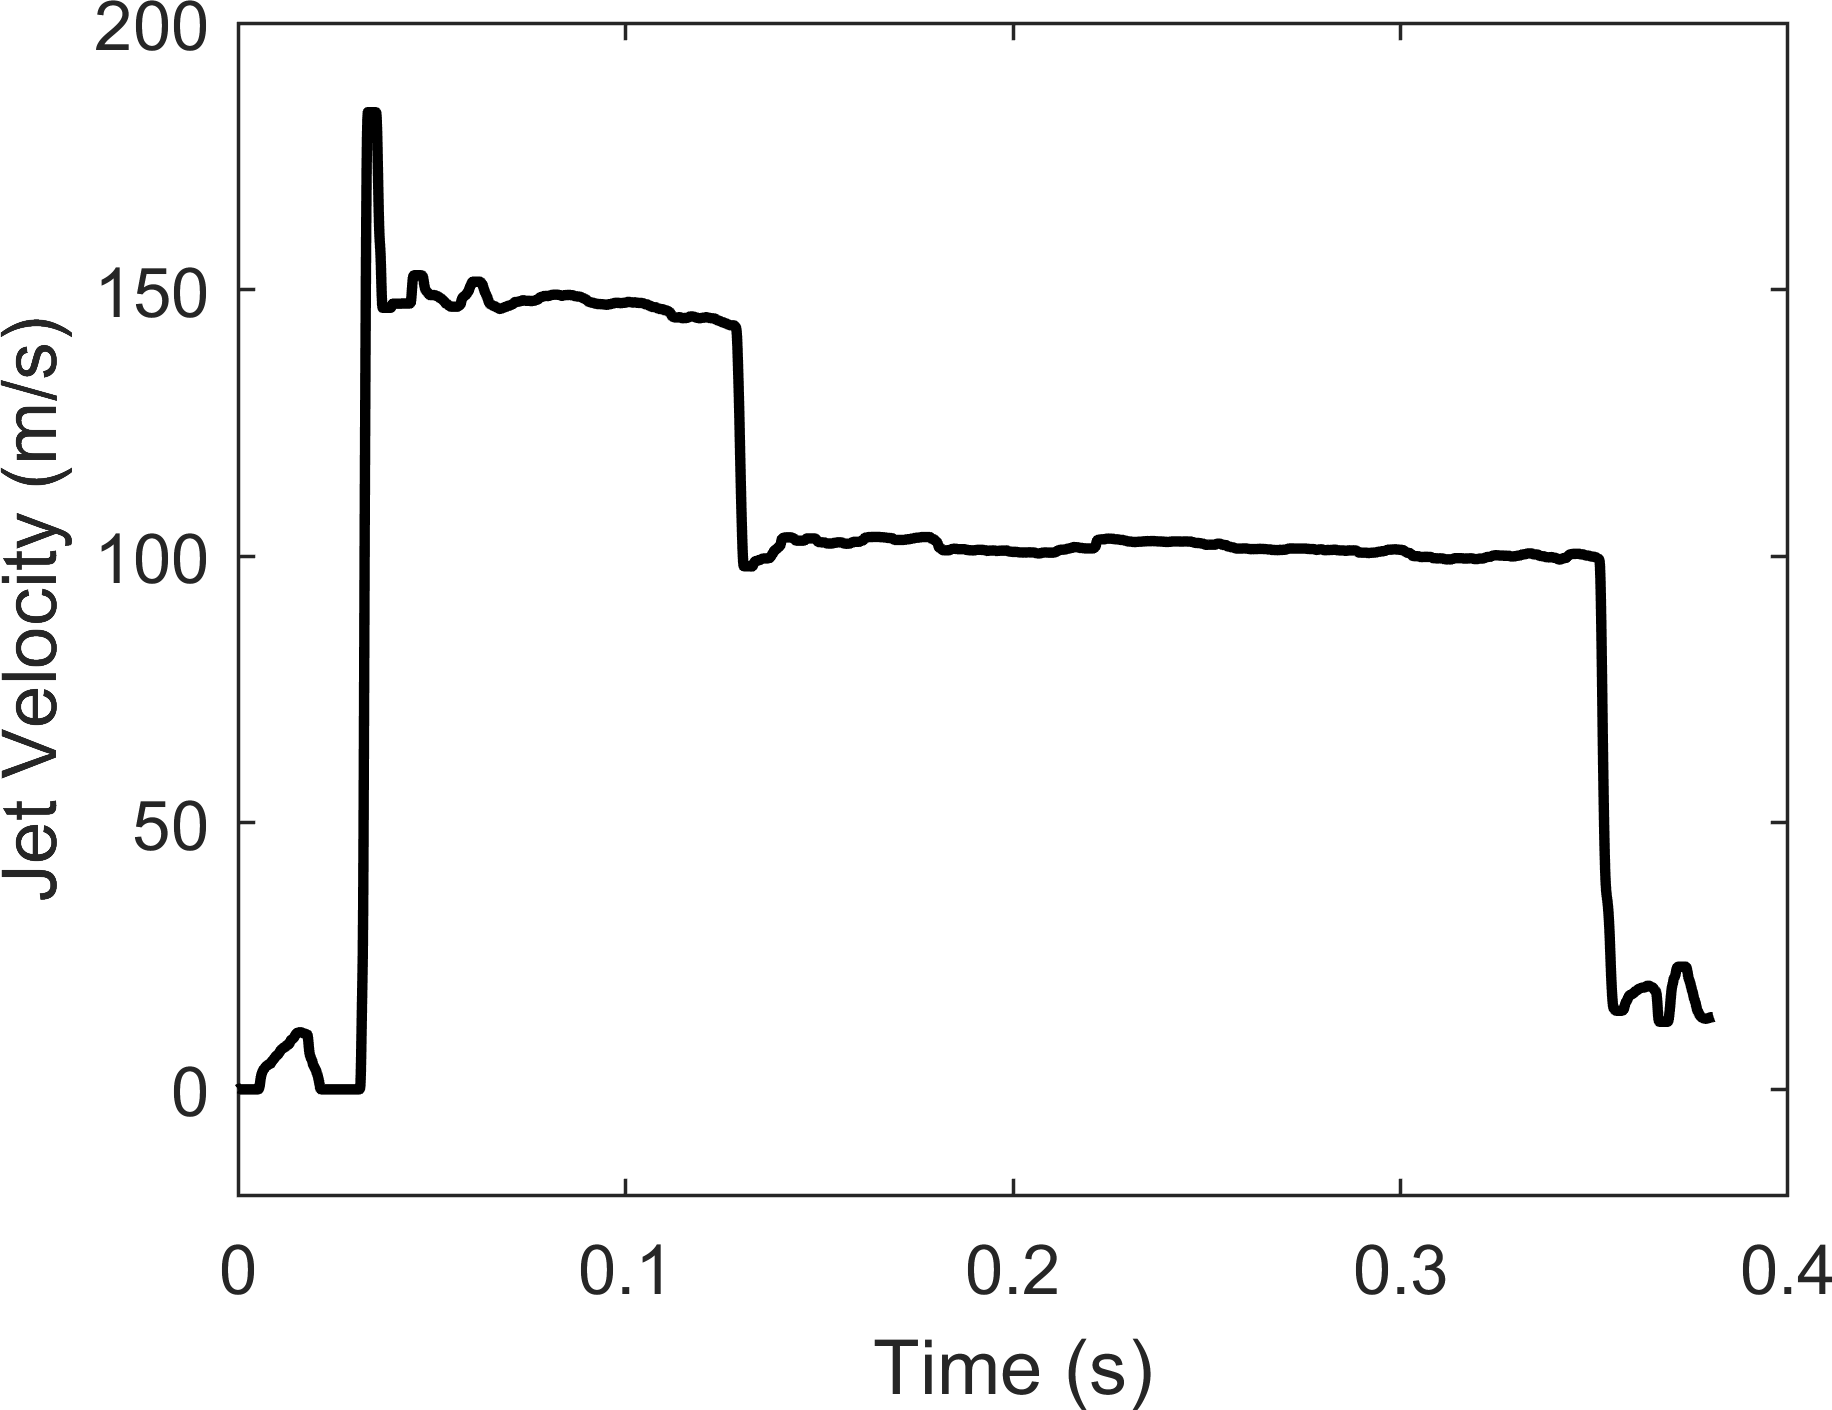
\includegraphics[width=3.4in]{chap5/images/injection_velocity_waveform_2_phase.png}
                \caption{Demonstration of 2 speeds injection: $v_{jet1}=150\,\mathrm{m/s}$ for the duration of $t_1=100\,\mathrm{ms}$, and then $v_{jet2}=100\,\mathrm{m/s}$ for the duration of $t_2=200\,\mathrm{ms}$}
                \label{fig:chap/experiment/injection_test/injection_velocity_waveform_2_phase}
            \end{figure}
        
        
            To demonstrate the speed control capability of the \acs{NFJI} system, an additional experiment was conducted. The closed loop velocity-controlled system was programmed to move to piston filled with water at the speed of $v_{jet1}=150\,\mathrm{m/s}$ for the duration of $t_1=100\,\mathrm{ms}$, and then at the speed of $v_{jet2}=100\,\mathrm{m/s}$ for the duration of $t_2=200\,\mathrm{ms}$. Fig.\,\ref{fig:chap/experiment/injection_test/injection_velocity_waveform_2_phase} plots the measured jet velocity over time from the sensor force measurement. The average jet profile though has shown overshoot still quickly settles toward $v_{jet1}=150\,\mathrm{m/s}$. The transition to $v_{jet2}=100\,\mathrm{m/s}$ was very smooth. Even though the system has some difficulty with piston position-control, it excels in velocity control. This experiment proved that the \acs{NFJI} system and especially the \acs{PMLSM} prototype as the whole is capable of delivering high volume and real-time velocity-controlled needle free jet injection.
        
        
        % -----------------------------------------------------------------------------------
        % --- NEW SUB SECTION --- NEW SUB SECTION --- NEW SUB SECTION --- NEW SUB SECTION ---
        % -----------------------------------------------------------------------------------
        \subsection{Injection test into tissue}              \label{Chapter:experiment/validation/injection test in tissue}
        
        
            \begin{figure}[!ht]
            	\centering
            	\subfloat[Injection test labelled "1"]{
            		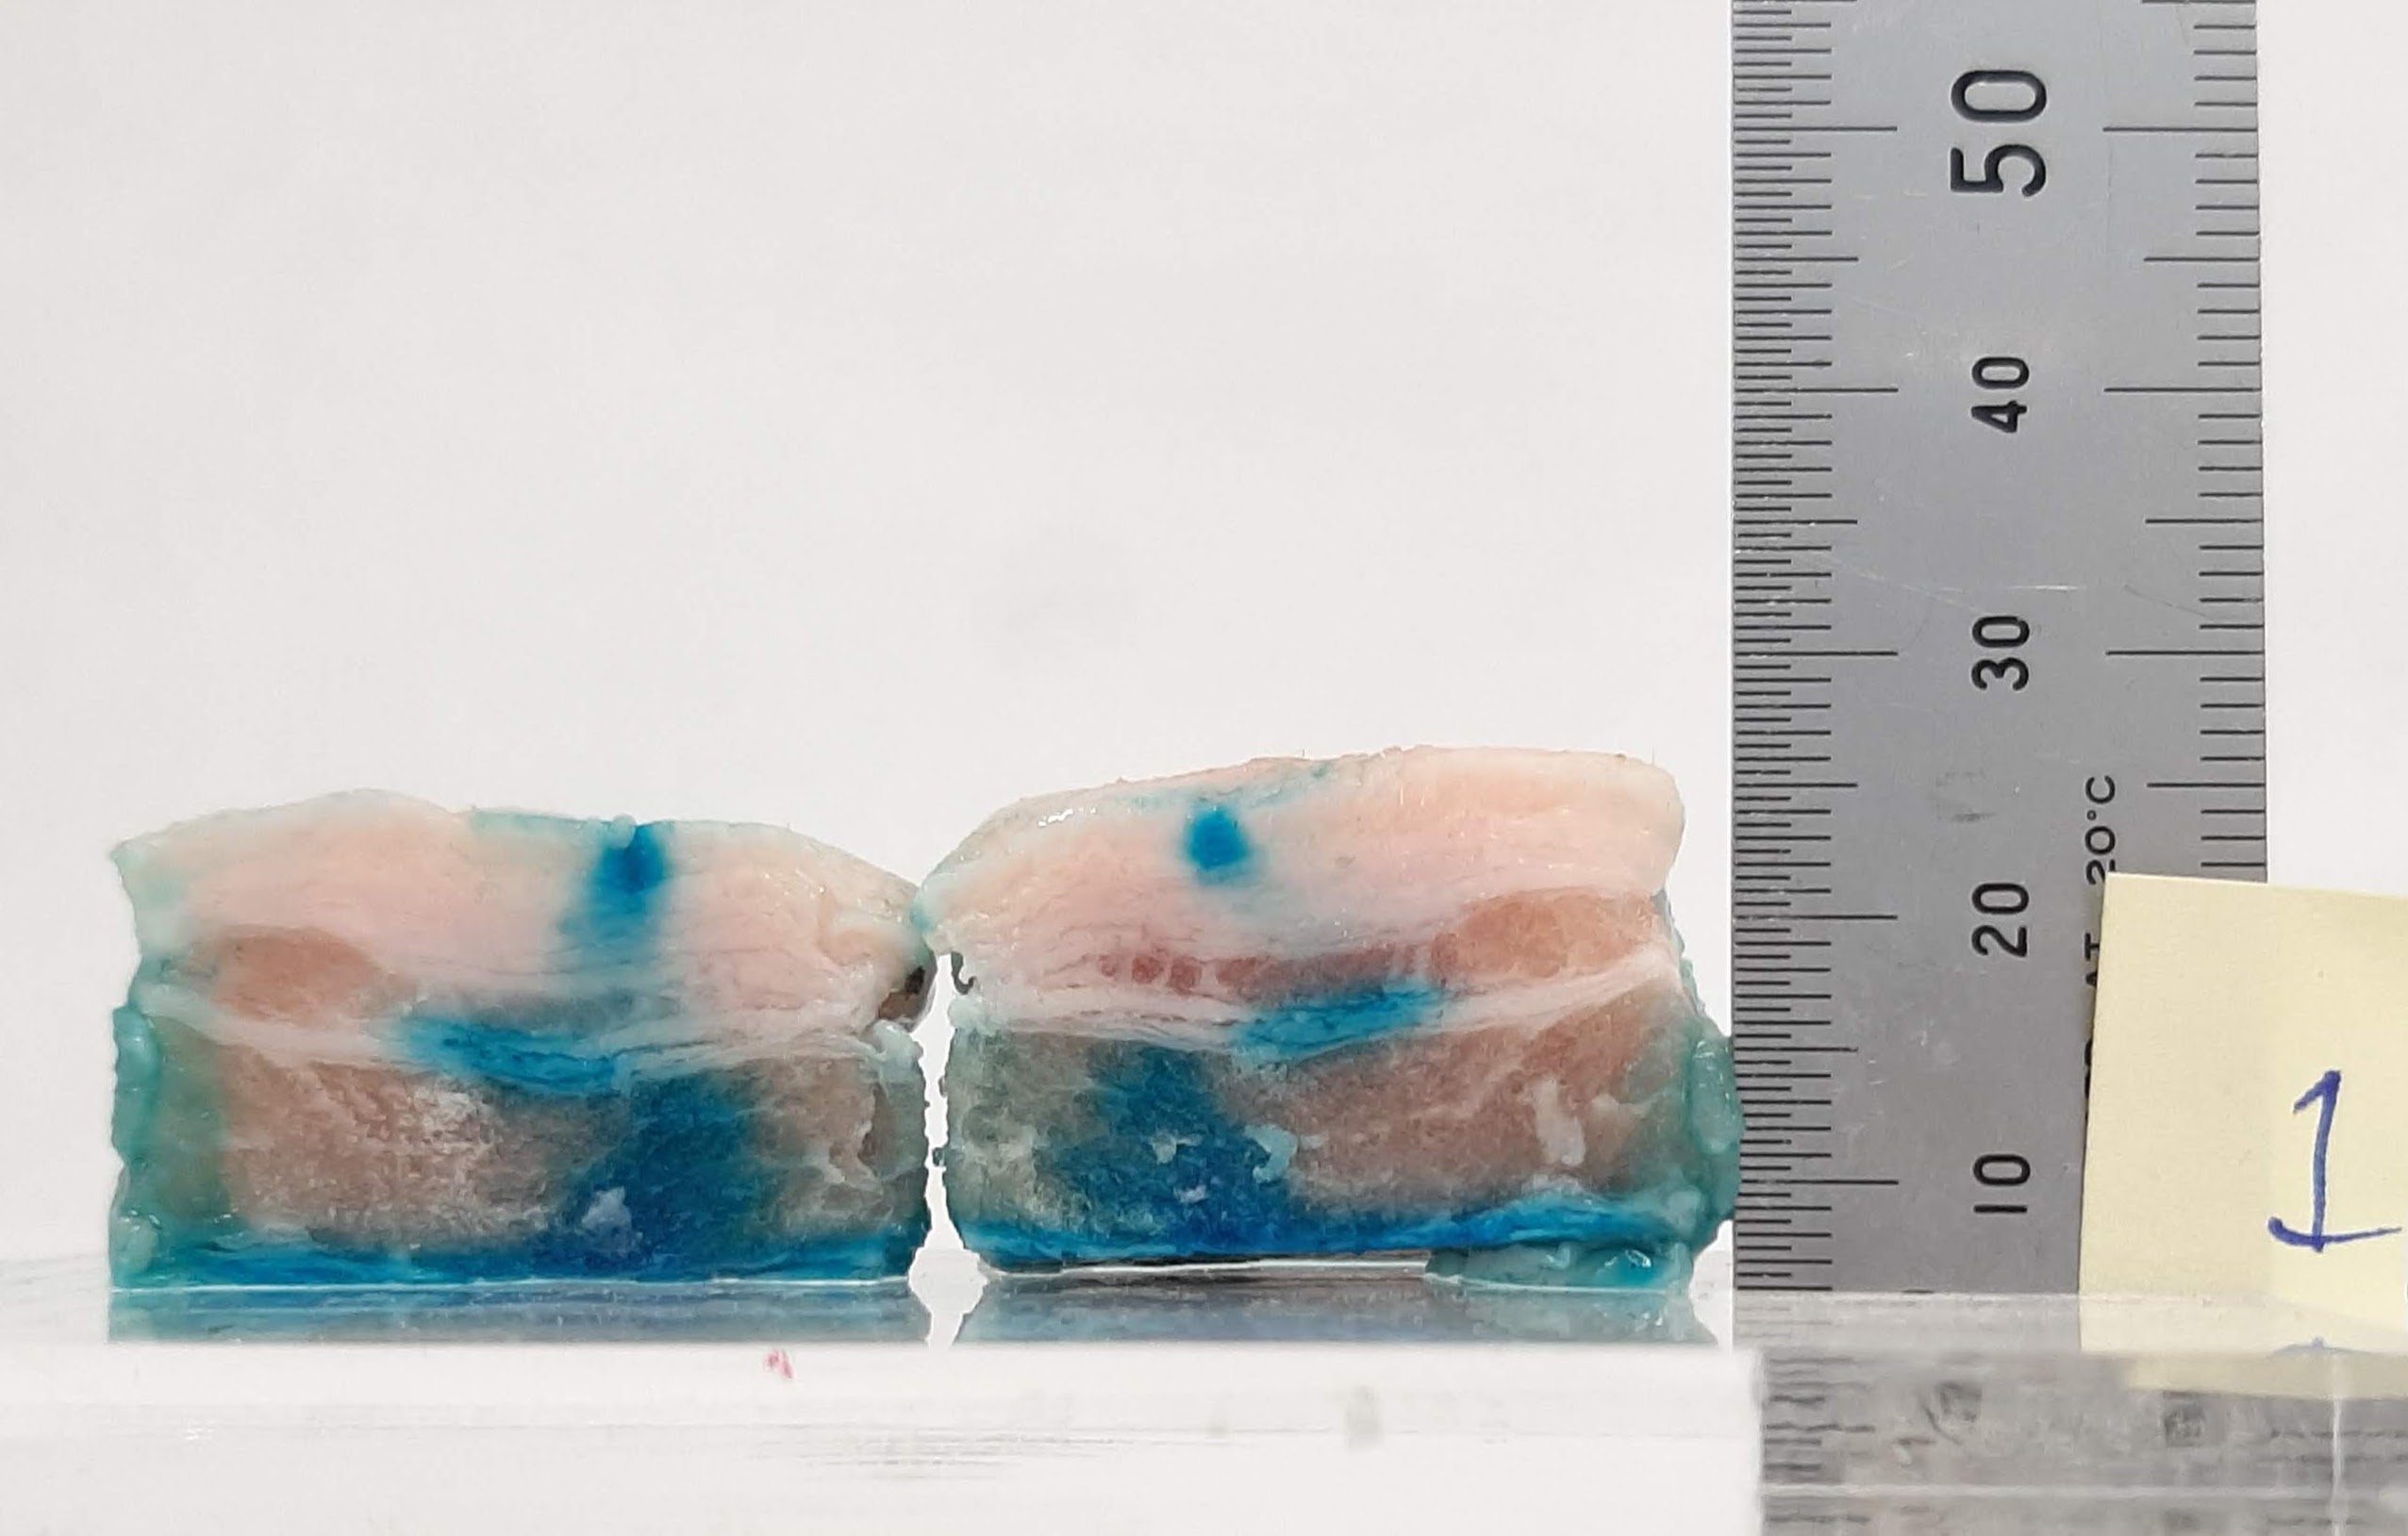
\includegraphics[width=3in]{chap5/images_exp/injection_label_1.jpg}
            		\label{fig:chap/experiment/injection_test_tissue/1}
            	}
            	\\
            	\subfloat[Injection test labelled "3"]{
            		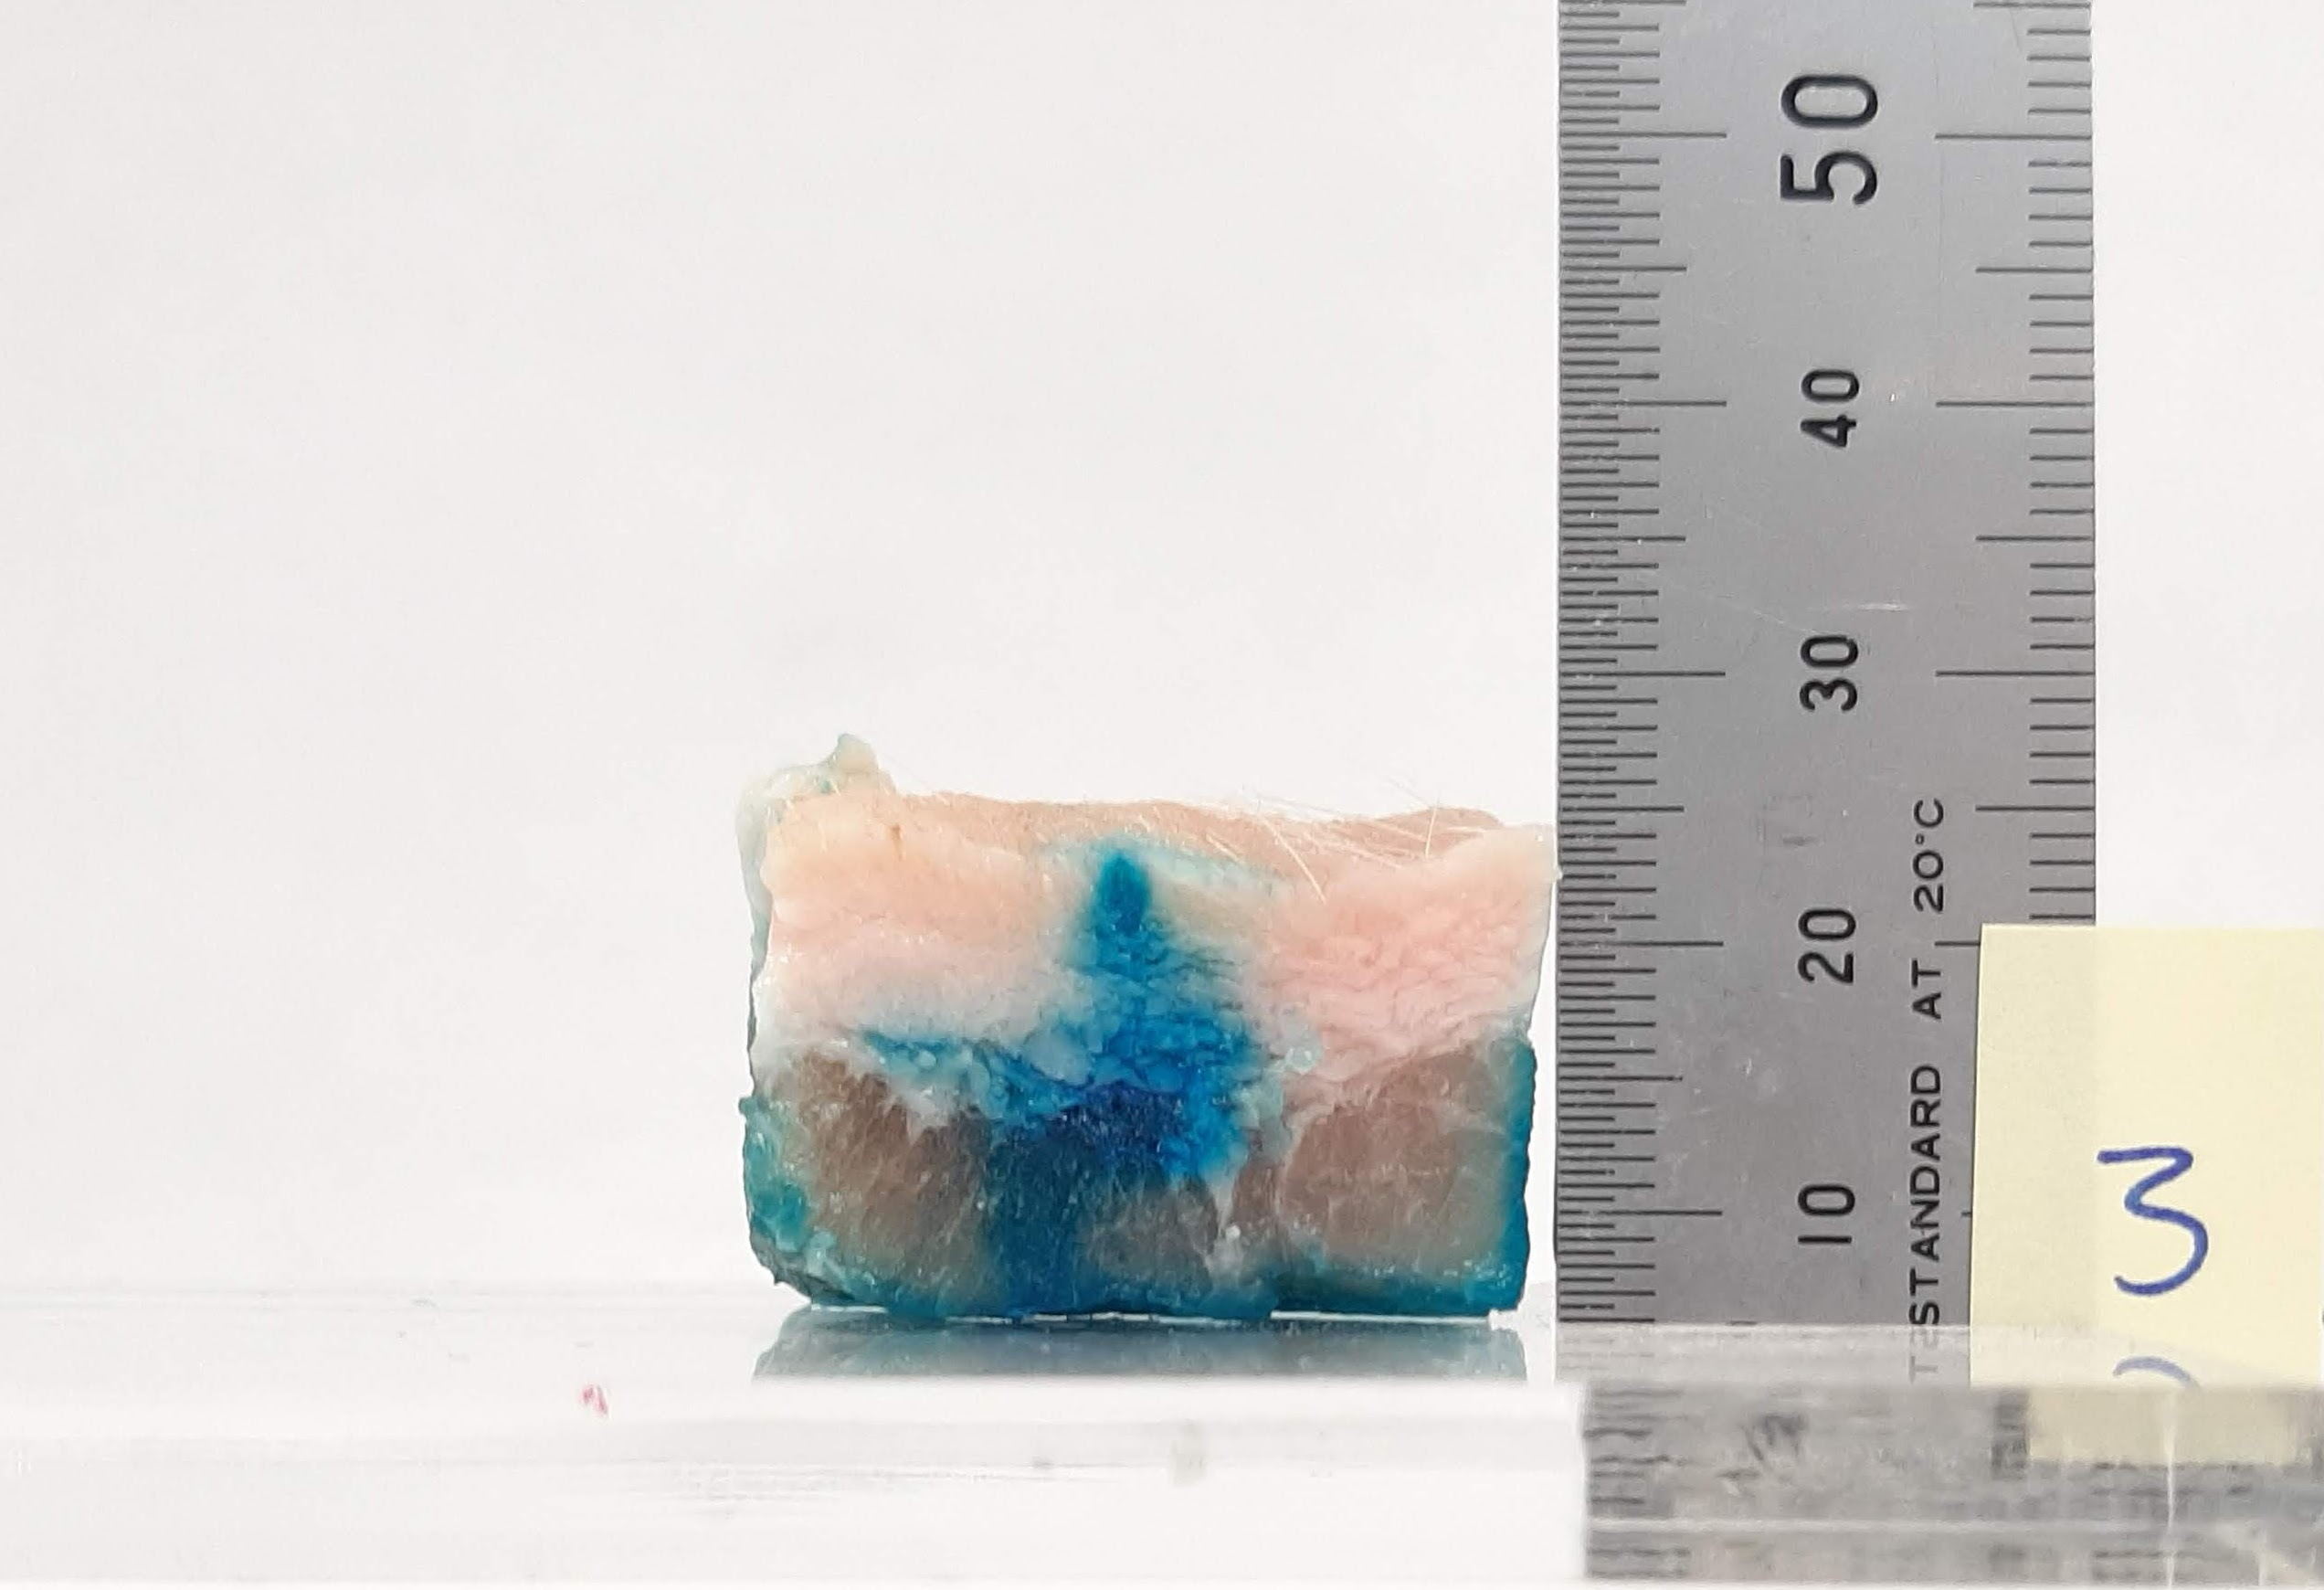
\includegraphics[width=3in]{chap5/images_exp/injection_label_3.jpg}
            		\label{fig:chap/experiment/injection_test_tissue/3}
            	}
            	\\
                \subfloat[Injection test labelled "5"]{
            		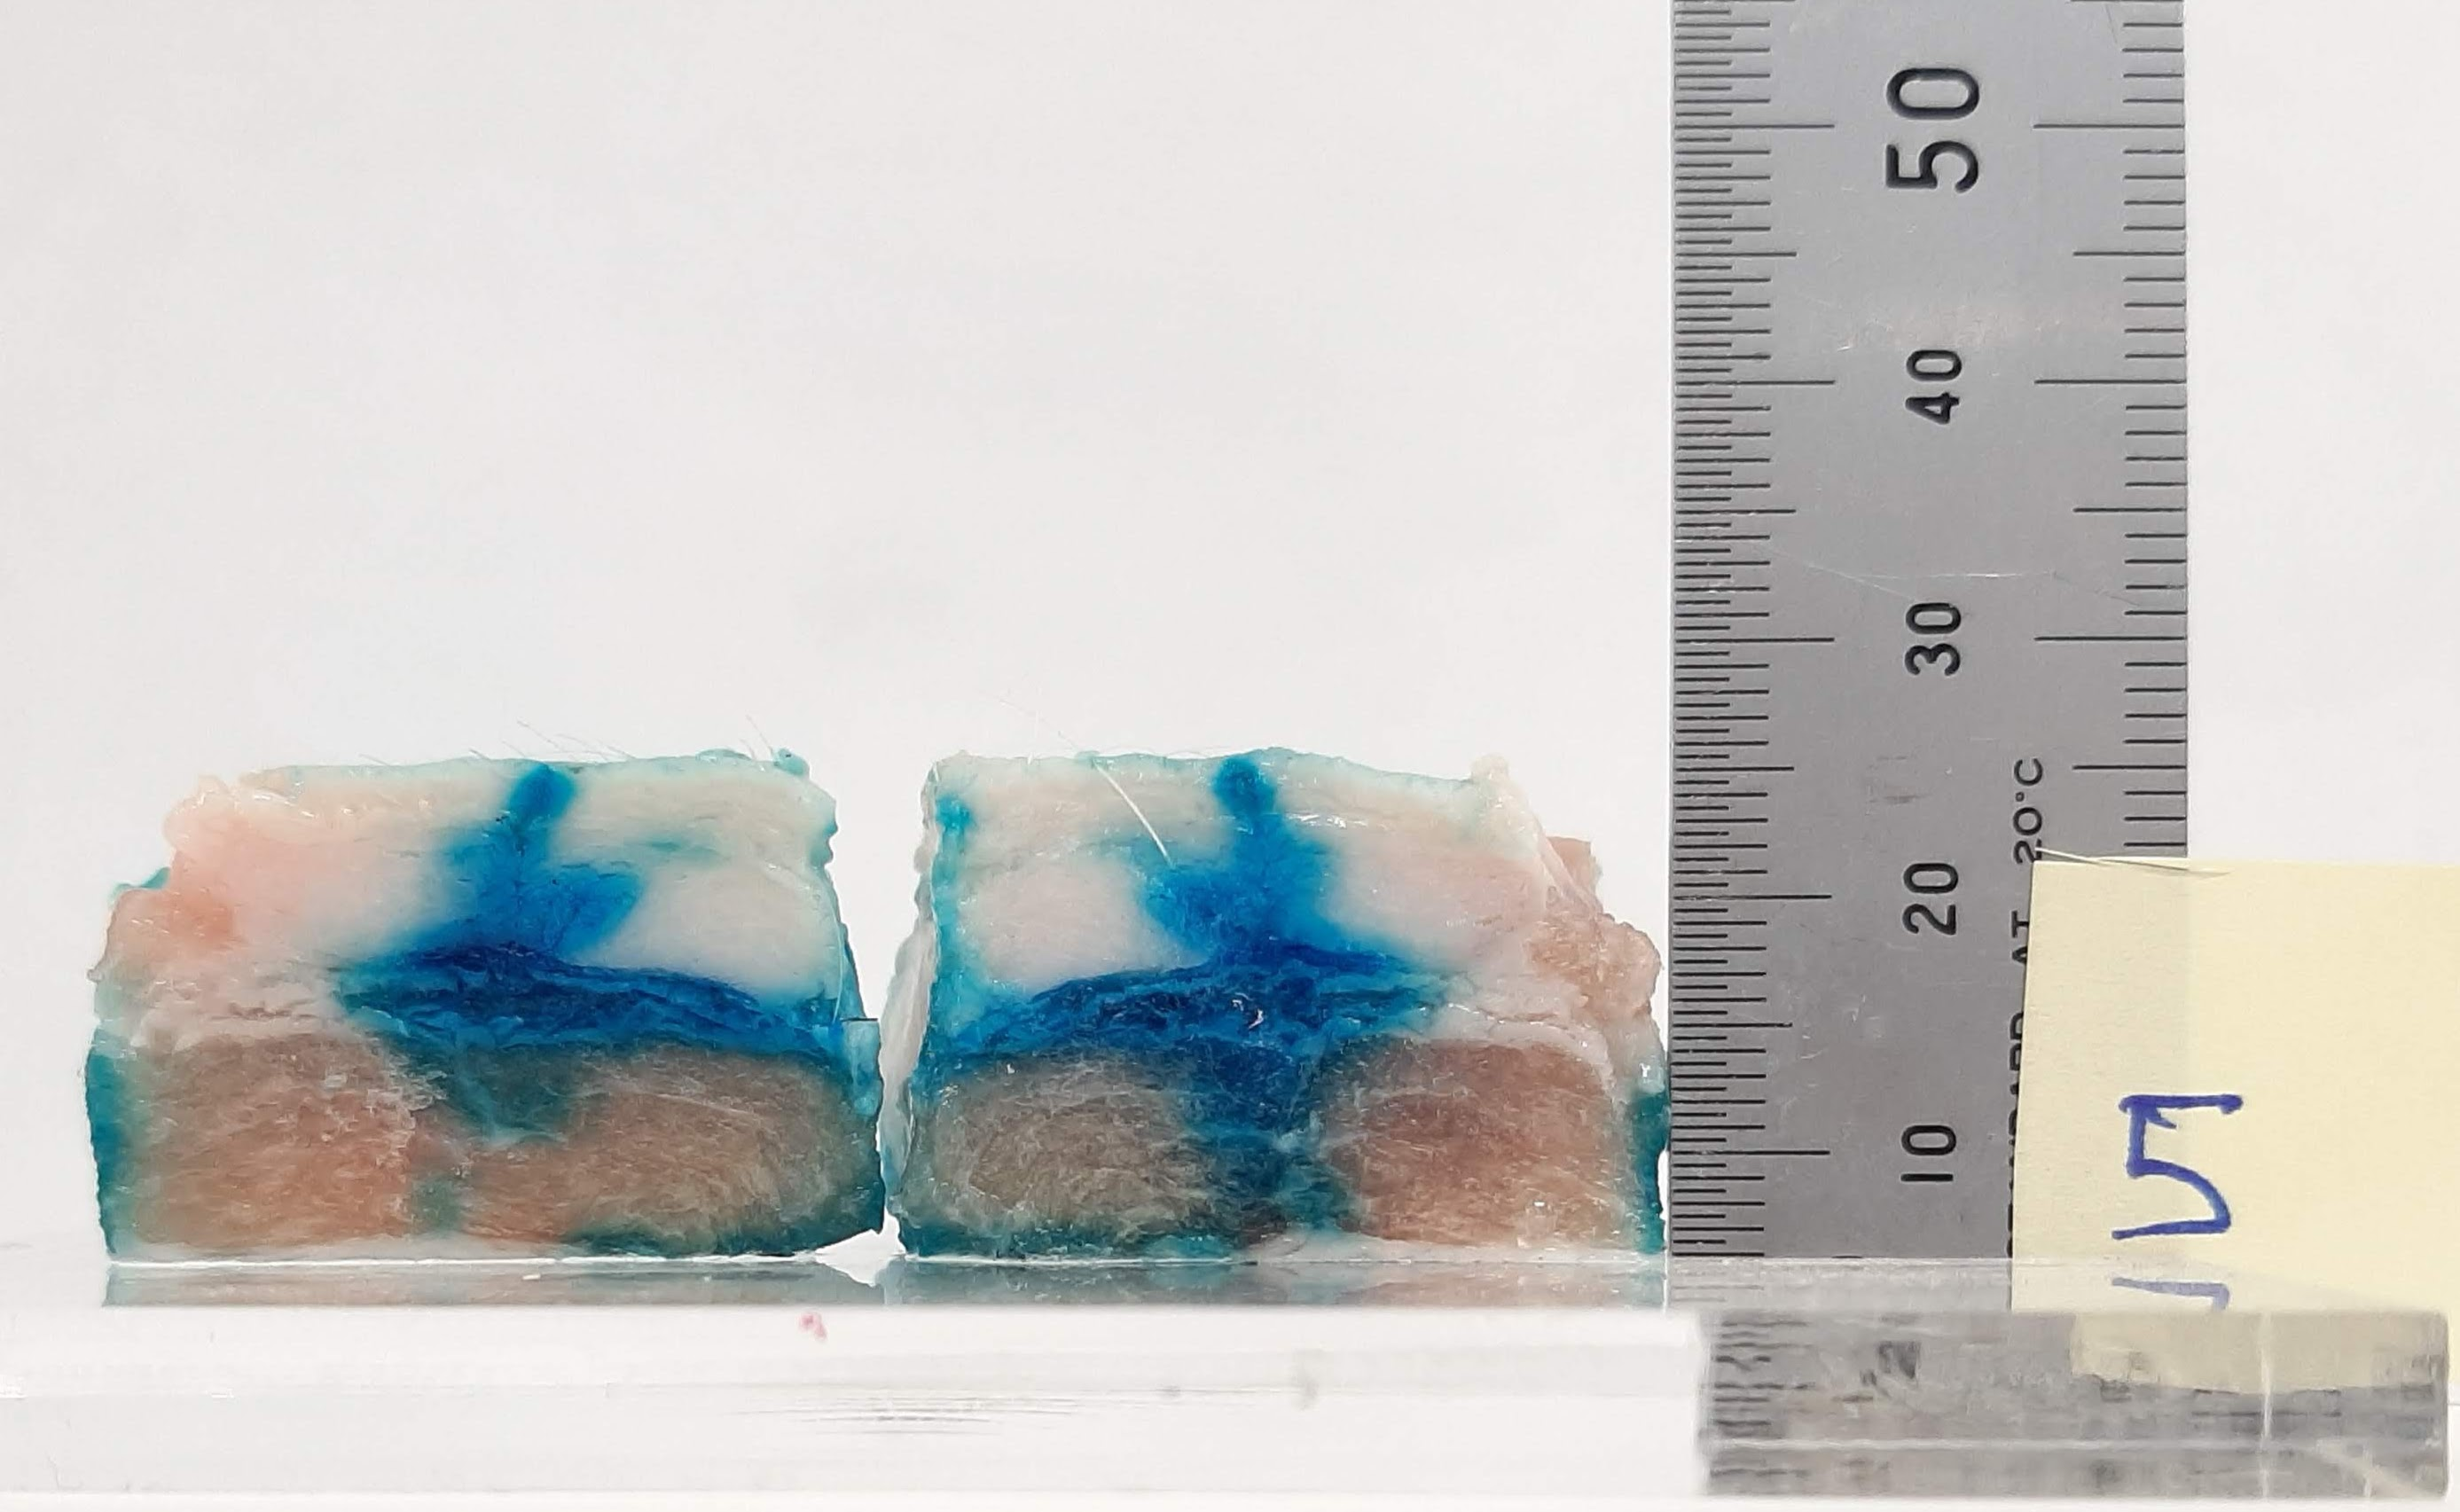
\includegraphics[width=3in]{chap5/images_exp/injection_label_5.jpg}
            		\label{fig:chap/experiment/injection_test_tissue/4}
            	}
                \caption{Results from two-phase jet injection into tissue: images of samples which have been injectioned, frozen and sectioned.}
                \label{fig:chap/experiment/injection_test_tissue}
            \end{figure}
        
        
            Injections were performed into $3\,\mathrm{cm} \times 3\,\mathrm{cm}$ cubes of porcine tissue harvested post-mortem from the abdomen animals of approximately 3 months of age. The tissue was obtained in compliance with the University of Auckland Code of Ethical Conduct for the Use of Animals for Teaching and Research. The porcine tissues included skin, subcutaneous fat and the foremost muscle layer, and were frozen and stored at $-80^{\circ}\mathrm{C}$. Prior to the injections, three samples were left at room temperature of roughly $~22^{\circ}\mathrm{C}$ for 4 hours. Each injection was performed using water with $0.1\,\%$ blue dye (Brilliant Blue FCF, Queen Fine Foods Pty. Ltd.) to allow visualisation of the destination of the injected liquid.
            
            
            The jet injector device were programmed to deliver colored water at the speed of $v_{jet1}=150\,\mathrm{m/s}$ for the duration of $t_1=100\,\mathrm{ms}$, and then at the speed of $v_{jet2}=100\,\mathrm{m/s}$ for the duration of $t_2=150\,\mathrm{ms}$. The expected volume to be delivered is $V=0.9375\,\mathrm{mL}$. Fig.\,\ref{fig:chap/experiment/injection_test_tissue} displays images of the samples which have been injected, frozen, then sectioned. The average rate of volume delivery is sitting very high at $85.7\,\%$. In all the tests, there are clear evidences that that the liquid all dispersed in between the fat and the muscle layers. Further than that, the drug penetrated all the way down into the muscle layer. One should note that the actual volume expended in the table was calculated based on how far the piston has traveled down the drug ampoule. Table\,\ref{table:chap/validation/exp/injection_into_tissue} summarizes the \acs{NFJI} delivery results for each of the samples in Fig.\,\ref{fig:chap/experiment/injection_test_tissue}.
            
            
            \begin{table}[h]
                \renewcommand{\arraystretch}{1.2}
                \caption{Summary of jet injection into tissues}
                \label{table:chap/validation/exp/injection_into_tissue}
                \centering
                \begin{tabular}{c|cccc|r}
                \hline
                \textbf{Sample} & \textbf{Weight of tissue} & \textbf{Weight of tissue} & \textbf{Volume}     & \textbf{Volume} & \% \textbf{volume}  \\
                             & \textbf{before injection} & \textbf{after injection}  & \textbf{delivered}  & \textbf{expended}        & \textbf{delivered}\\
                \hline
                "1"          & $32.31\,\mathrm{g}$               & $33.11\,\mathrm{g}$              & $0.80\,\mathrm{mL}$ & $0.94\,\mathrm{mL}$      & $85.1\,\%$          \\
                "3"          & $32.16\,\mathrm{g}$               & $32.97\,\mathrm{g}$              & $0.81\,\mathrm{mL}$ & $0.96\,\mathrm{mL}$      & $84.4\,\%$          \\
                "5"          & $32.18\,\mathrm{g}$               & $33.02\,\mathrm{g}$              & $0.84\,\mathrm{mL}$ & $0.97\,\mathrm{mL}$      & $86.6\,\%$         \\
                \hline
                \end{tabular}
            \end{table}
        
        
        % -----------------------------------------------------------------------------------
        % --- NEW SUB SECTION --- NEW SUB SECTION --- NEW SUB SECTION --- NEW SUB SECTION ---
        % -----------------------------------------------------------------------------------
        \section{Discussion}                     \label{Chapter:experiment/validation/discussion}
        
        
            To summarize, this work utilized the modeling method presented in Chapter\,\ref{Chapter:PMLSM design HM} and a new optimization methodology to find a globally optimized motor configuration for NFJI that is complemented by an iron length that produces the minimal amount of cogging. The motor was designed to deliver $1\,\mathrm{mL}$ NFJIs, at rated motor speed of $0.5\,\mathrm{m/s}$, rated force of $250\,\mathrm{N}$, and rated electrical power requirement of $1.2\,\mathrm{kW}$. 
            
            
            The measured motor constant, peak-to-peak cogging force, and bearing friction of the prototype motor constructed corresponding to the optimized design were $6.6\,\mathrm{N/\sqrt{W}}$, $4\,\mathrm{N}$ and $4.2\,\mathrm{N}$, respectively. Based upon the voltage constants and the phase resistance measurements, the motor constant found was within $10\,\%$ of the design value of $7.2\,\mathrm{N/ \sqrt{ \mathrm{W}}}$. This reflects a good modelling result, although the modelling accuracy could be still be improved by tightening the modelling assumptions. 
            
            
            Together with the weights of the support structure and all related parts to contain and delivery the drug, the hand piece weighs $622\,\mathrm{g}$. The first place to look at to reduce the weight for the hand piece device would be the current aluminium drug ampoule. While rigid and robust, the drug amouple would be replaced with  poly-carbonate to save $60\,\%$ weight on this part without compromising the structure rigidity. From then, one can look at optimizing the weight of the support plate and rods. 
            
            
            In a test injection provided with $1.4\,\mathrm{kW}$ of electrical power, the prototype motor produced a $200\,\mathrm{\mu m}$ thin jet of water into a force sensor with an average jet velocity of $134\,\mathrm{m/s}$, well within the practical jet injection velocity range \cite{mitragotri2006}. Thereby, this prototype successfully demonstrated the capability for large volume needle-free jet injection. The \acs{NFJI} system performed not so well in closed loop position control mode but very well in speed control mode as illustrated in Fig.\,\ref{fig:chap/experiment/injection_test/injection_test} and \ref{fig:chap/experiment/injection_test/injection_velocity_waveform_2_phase}. In three injection tests into porcine tissue, the average volume delivery rate was $85.7\,\%$ which demonstrated the repeatability and realiablity of the \acs{NFJI} system powered by \acs{PMLSM}. Future effort could aim at system advanced identification and improvement for closed loop position control. 
            
            
            It is also worth mentioning that it is possible for the prototype motor to employ a compound ampoule similar to that reported in \cite{Ruddy2015a,McKeage2018}, making the device capable of delivering close to\,$4\,\mathrm{mL}$ of liquid drug, and thus surpassing the volume needed for most protein based formulations \cite{Hogan2015}.